\chapter{ACP-HCS interaction in \bet-branching}
\label{cha:ACP-HCS}

\section{Introduction}
\label{sec:IntroACP-HCS}
Some type I Polyketide biosynthesis systems, for example producing mupirocin, thiomarinol, kalamanticin, or myxovericins, are found to incorporate a branch on the third (i.e. \bet) carbon in the growing polyketide chain, referred to as a \bet-branch. This \bet-branching mechanism is thought to be catalysed via an \textquotedblleft HMG-CoA synthase (HCS) cassette\textquotedblright, consisting of an HMG-CoA synthase homologue and further auxiliary enzymes. In the mupirocin system the HCS cassette is a set of 5 proteins of which MupH (the HMG-CoA synthase homologue) is the first enzyme to interact with an acyl carrier protein (ACP) from the MmpA subunit. This interaction between ACP and MupH initiates the \bet-branching reaction. 

At the start of the present work little was known about the HCS cassette structure and function or how it interacts with the proteins in PKS? It was not understood what allows MupH to recognize the ACPs with substrates for \bet-branching, as opposed to the several other ACPs involved in a typical PKS pathway where branching is not required. We also did not know whether HCS proteins have a subtype or if they always work as one set of only five proteins as found in the mupirocin cluster. However, a recent study of the myxovirescin system \parencite{Simunovic2006} shows two HCS clusters involved in \bet-branching at two position in the synthesis pathway. These two stages are catalysed by two non-complimentary pairs of HMG-CoA synthase homologue and ACP interactions, which suggests the possibility of HCS subtypes. In a study of the curacin system, it was found that the HCS proteins can also work in conjunction with a halogenase. This halogenase activity adds a halogen (chlorine in case of curacin) on the $4^{th}$ ($ \gamma $-carbon) carbon of the growing polyketide chain \parencite{Busche2012}. 

A number of questions arise.
\begin{inparaenum}[\itshape 1\upshape)]
\item How different are the ACPs which interact with the HCS cassette from other ACPs found in the pathway? 
\item Is it possible to predict the molecular features responsible for the ACP-HCS recognition? 
\item And can these molecular features be exploited for the engineering of \bet-branching function in mupirocin biosynthesis pathway or other systems?
\end{inparaenum}
I have used computational methods to address these exciting questions. The work started using the preliminary data available from Prof. Christopher M. Thomas lab. 

In a sequence analysis carried out by Dr. Anthony Haines on the ACPs from various PKS systems, in \bet-branching ACPs a conserved tryptophan motif is found (Figure \ref{fig:WflagAlignment}) at the position 6 residues downstream of the catalytic serine. This position is not found to be conserved in the non-branching ACPs. It was also found that upon mutating this conserved tryptophan to leucine in the mupirocin system the production of pseudomonic acid A is significantly lowered. Thus, it was hypothesized that this conserved tryptophan could be the recognition motif. These preliminary observations lead Dr. Mathew Crump from the University of Bristol to solve the solution structure of the ACP di-domain from module 6 of the MmpA subunit in the mupirocin biosynthesis pathway. This NMR structure (PDB ID 2L22) has been used in the present work to carry out the predictions on the ACP-HCS interaction mechanism.

	\subsection{HMG-CoA synthase cassette}
	\label{sec:HMG-Coasynthase}
	The HCS cassette in the mupirocin biosynthesis pathway, is a set of 5 proteins consisting of an ACP (mACPc), a 3-hydroxy-3-methylglutaryl-CoA (HMG-CoA) synthase homologue (MupH), a decarboxylase (MupG) and two proteins (MupJ, MupK) from the crotonase superfamily. MupH homologues, our focus here \parencite{Wu2007}, are found in various polyketide biosynthesis pathways and are thought to be involved in \bet-branching mechanisms along with the other enzymes in the HCS cassette. It is hypothesized that acyl carrier proteins from the ACP di-domain (ACP-mupA3a and ACP-mupA3b), in the MmpA subunit of the mupirocin biosynthesis pathway, make the first point of contact with the MupH, initiating the \bet-branching reaction. This interaction between the ACPs and MupH is thought to be governed by a set of specificity determinants in the interacting residue pairs, which allows the ACPs involved in the \bet-branching systems to recognise and interact with the proteins in the HCS cassette. To understand better what governs the interaction between the ACPs and MupH, a structural model of the ACP-mupH complex determined either through experimental or computational methods could help to design mutagenesis experiments. The solution structure for the ACP-mupA3ab di-domain has been recently resolved (PDB ID 2L22), however there is no structure available for MupH. To predict a reliable structure of MupH and to understand its structural properties it was necessary to first understand the structural properties and the reaction mechanism catalysed by its homologue HMG-CoA synthase.

		\subsubsection{HMG-CoA synthase reaction mechanism}
		\label{sec:HCSreact}
		HMG-CoA synthases (EC 2.3.3.10) are 42 KDa proteins found in a wide range of organisms from bacteria to mammals and play a central role in fatty acid, polyketide, and isoprenoid biosynthesis. The enzyme belongs to the thiolase superfamily and can be broadly classified into the bacterial isoforms, the eukaryotic cytosolic isoforms and the mammalian specific mitochondrial isoform \parencite{Shafqat2010}.
	
		HMG-CoA synthase catalyses a three step reaction that involves a conserved Cys-His-Glu catalytic triad and an acyl-enzyme intermediate. As in \textit{Enterococcus faecalis} HMG-CoA synthase (PDB Id 1X9E) the first step is a \textbf{deacetylation} of the substrate Ac-CoA, H233 is thought to act as a catalytic base or H-bond donor for the nucleophilic C111, which attacks the carbonyl carbon of Ac-CoA , thereby transferring the acetyl group to the Cys-S atom and releasing the reduced CoASH (Figure  \ref{fig:HMGCO-Areact}) \parencite{Steussy2005}.

		\setlength\fboxsep{5pt}
		\setlength\fboxrule{1.5pt}
		\begin{figure}[]
		\centering
		\fbox{\includegraphics[width=0.9\textwidth, keepaspectratio=true]{graphics/hmgreact.pdf}}
		\caption[The reaction mechanism of HMG-CoA synthase.]{The reaction mechanism of HMG-CoA synthase. proposed in \parencite{Steussy2005}}.
		\label{fig:HMGCO-Areact}
		\end{figure}				
	
		In the second step, the methyl group of acetylated-Cys is deprotonated by the general base G79 to form a carbanion which attacks the distal (\bet) carbonyl of the incoming AcAC-CoA (second substrate), following the \textbf{condensation} of Ac-Co and AcAC-CoA forming an enzyme:HMG-CoA intermediate.
	
		In the final step the resultant enzyme:HMG-CoA intermediate is \textbf{hydrolyzed} to release the product HMG-CoA and regenerate the reduced Cysteine. G79 is shown to mediate the hydrolysis step. The similar reaction mechanism is also observed in \textit{Staphylococcus aureus, Brassica juncea} and Human HMG-CoA synthases \parencite{Theisen2004, Shafqat2010}.
		
		It is assumed that the \bet-branching mechanism of MupH would be similar to that of HMG-CoA synthase and thus can be used to guide the modelling.

\section{Results}

	\subsection{ACP sequence analysis}
	\label{sec: ACPSequenceAnalysis}
	The initial sequence analysis carried out by Dr. Anthony Haines on the seven well-characterized PKS clusters known to be involved in \bet-branching (Figure \ref{fig:WflagAlignment}) revealed the presence of a conserved tryptophan 6 residues downstream of the catalytic serine. A W was not seen at this position in the non-branching ACPs. Dr. Haines further used the sequence motif (DSXXXXXW) as a search pattern for PHI-BLAST and found further ACPs that he confirmed from the literature were associated with \bet-branching \parencite{Haines2013}. This sequence motif predicted ACPs from all the known systems involved in \bet-branching with the exception of two ACPs from virginiamycin and leinamycin clusters each. Which suggests that although this sequence motif is a strong predictor of \bet-branching associated ACPs it might not be enough to predict all of them. Therefore in the present study a stronger predictor, based on the statistical method of Hidden Markov models (HMM), was developed to classify ACPs into \bet-branching and non-\bet-branching types.
	
	\setlength\fboxsep{5pt}
	\setlength\fboxrule{1.5pt}
	\begin{figure}[]
	\centering
	\fbox{\includegraphics[width=0.9\textwidth, resolution=600, keepaspectratio=true]{graphics/wflagalignment.png}}
	\caption[Alignment of the ACP sequences from HCS cassette containing systems.]{Alignment of the ACP sequences from HCS cassette containing systems provided by Dr. Anthony Haines. The conserved W is indicated by a *.}
	\label{fig:WflagAlignment}
	\end{figure}
		
	 The sequences provided by Dr. Anthony Haines were used to build HMMs using 38 and 178 sequences from 15 well characterised pathways for the \bet-branching and non-\bet-branching ACPs respectively. These models were tested using a test set of ACPs (provided by Dr. Anthony Haines) from other clusters which were not part of the training set. These results were plotted on a graph of non-\bet-branching HMM score against \bet-branching HMM score (Figure \ref{fig:hmmplot}). The graph was divided by the $y=x$ line where the models predict an ACP as having the same likelihood of being a \bet-branching ACP or standard ACP. The majority of ACPs from the remaining clusters with at least one identified \bet-branch-associated ACP locate to one or other of these clusters (Figure \ref{fig:hmmplot}). 
	 
	 \bet-branching ACPs from the virginiamycin cluster were identified as the outliers which are just above the $ y=x $ line and adjacent to the \textquoteleft branching\textquoteright{ } cluster. Other outliers were the two \bet-branching ACPs from the leinamycin cluster one of which was just below the line and the other actually fallen within the non-branching cluster. Except for leinamycin, classifying ACPs using HMMs agrees with the available information about their likely presence in the \bet-branching or non-\bet-branching modules. The model for non-\bet-branching ACPs (standard) was used to fetch the ACP sequences from the UniProtKB/TrEMBL (20127441 seq) and Refseq microbial (6408654 seq) databases, database version on 9th March, 2012. I developed a couple of Perl scripts (see Appendix I) to remove all the sequences which were shorter than 60 aa or duplicates or sequences without the phosphopantethinylated serine which resulted in a set of 16,490 unique sequences. To ensure that these sequences cover the full length of the model, they were extended by 7 residues on both the ends. The extended sequences were scored using both the HMM models and a scatter diagram was plotted (Figure 3. Scatter diagrams showing the separation of ACPs into two clusters by their fit to the \bet-branch-associated \textquoteleft branching\textquoteright{ } ACP HMM and the non-branching \textquoteleft standard\textquoteright{ } ACP HMM. (b)). In Figure  \ref{fig:hmmplot} the scatter plots shows the separation of ACPs into two clusters by their fit to the \bet-branch-associated \textquoteleft branching\textquoteright{ } ACP HMM and the non-branching \textquoteleft standard\textquoteright{ } ACP HMM. These scatter plots were rendered by Dr. Anthony Haines using the data provided by the HMM analysis carried out by Rohit Farmer (this graph is also presented in \parencite{Haines2013}). 

	\setlength\fboxsep{5pt}
	\setlength\fboxrule{1.5pt}
	\begin{figure}[]
	\centering
	\fbox{\includegraphics[width=0.9\textwidth, resolution=600, keepaspectratio=true]{graphics/hmmplot.png}}
	\caption[Scatter diagrams showing the separation of ACPs into two clusters by their fit to the \bet-branch-associated ‘branching’ ACP HMM and the non-branching ‘standard’ ACP HMM.]{Scatter diagrams showing the separation of ACPs into two clusters by their fit to the \bet-branch-associated ‘branching’ ACP HMM and the non-branching ‘standard’ ACP HMM. (A) ACPs from 26 pks clusters with at least one known or predicted branching ACP. (\textcolor{PineGreen}{$ \square $}) Training set for HMM using known branching ACPs. (\textcolor{PineGreen}{$ \blacksquare $}) predicted branching except (\textcolor{PineGreen}{$ \blacktriangle $}) virginiamycin cluster branching ACPs and (\textcolor{PineGreen}{$ \times $}) leinamycin cluster \bet-branch-associated module ACPs (\textcolor{Thistle}{$\lozenge$}) Training set for HMM using non-branching ACPs (\textcolor{Thistle}{$ \blacklozenge $}) predicted non-branching ACPs. (B) 16,490 ACP-like sequences identified by screening the TrEMBL and RefSeq protein databases using the standard ACP HMM. Sequences which did not pass the branching HMM cut-off were conferred a score of 10 so they could be plotted. (\textcolor{PineGreen}{$ \blacklozenge $}) branching ACP. (\textcolor{PineGreen}{$ \blacksquare $}) unlisted variants in similar clusters (\textcolor{PineGreen}{$ \times $}) known branching, (\textcolor{PineGreen}{$ \blacktriangledown $}) predicted branching, identified in this screen (\textcolor{PineGreen}{$ + $}) ACPs which may add branches in a non-type I-pks pathway. (\textcolor{Dandelion}{\textbullet}) insufficient sequence context or conflicting information. (\textcolor{Thistle}{$ \blacktriangle $}) predicted non-branching ($ \cdotp $) not examined. Graph and parts of the figure legend copied from \textcite{Haines2013}.}
	\label{fig:hmmplot}
	\end{figure}
		
	The newly found ACPs in the screen could be classified as likely \bet-branching or non-branching. On the graph, close to the $ y=x $ line, an HMM score of above 45 represents the ambiguous regions where the branching state of an ACP cannot be predicted below 45 seems to be indicative of non branching. One ACP from the leinamycin cluster was found in this region, the other in the non-branching region. The two \bet-branching ACPs from the myxovirescin, cluster, which are associated with different MupH homologues, can be clearly identified. This suggests that the HMM model can be used to identify the ACPs associated with the \bet-branching but cannot be used to predict the ACP subtypes if they exist.
			
		\subsubsection{Minimum changes required to shift ACP-tmlD3a from non-\bet-branching to \bet-branching cluster.}
		\label{sec:MinumChanges}
		It was observed in the HMM analysis that the \bet-branching ACPs and the non-\bet-branching ACPs (standard) cluster in different zones, which raises a question as to the minimum changes necessary to shift an ACP from standard ACP cluster to \bet-branching ACP cluster, as scored by the HMM models? These mutations might allow us to make a non-branching ACP function like a \bet-branching ACP.
				
		To address this question I wrote a Perl script (Appendix I, Script \ref{sec:MinChangesScript}) to mutate each and every position in the sequence to the other 19 proteinogenic amino acids. A non branching ACP (ACP-tmlD3a) from the thiomarinol cluster was taken as the sequence of reference. ACP-tmlD3a was chosen because experiments from Prof. Thomas group showed no mupirocin production upon replacing ACP-mupA3a/b with ACP-tmlD3a/b. The script generated all possible substitutions at each of the 67 positions in the sequence, giving 19 X 67  = 1273 sequences.
	
		\setlength\fboxsep{5pt}
		\setlength\fboxrule{1.5pt}
		\begin{figure}[]
		\centering
		\fbox{\includegraphics[width=0.9\textwidth, resolution=600, keepaspectratio=true]{graphics/minchanges.pdf}}
		\caption[The number of mutations required to reach the score of 82.2 or above when scored with \bet-branching HMM model.]{The ACP-tmlD3a sequence scored 59.8 against \bet-branching HMM model and would require 5 mutations at the positions 6, 7, 11, 14 , and 20 counting from the active site serine (0) to reach the score 82.9 and 6$^{th}$ mutation at position 27 to score 85.7. Figure  3 .9 shows the relative positions of the residues required to be mutated on the ACP-tmlD3a:MupH complex}
		\label{fig:minchanges}
		\end{figure}
					
		From the previous analysis it was observed that the \bet-branching ACP sequences typically score in the range of 82.2 to 109.6 using \bet-branching HMM model (wacp.hmm). This suggests that if any sequence scores 82.2 or above using \bet-branching HMM model, should fall under the \bet-branching cluster. Utilizing this observation the 1273 sequences were scored using \bet-branching model %(wacp.hmm), 
		thus generating a first generation of mutated sequences. The sequence with the highest score was selected for the next generation of mutations and the process was iterated till a score of 82.2 or above was reached. For ACP-tmlD3a it took 5 generations (iteration) to reach the score of 82.9 and 85.7 in 6 generations. 
				
		This experiment suggests that it would need to make a minimum of 6 mutations at the positions shown in Figure \ref{fig:minchanges} and listed in Table \ref{tab:MinimumACPChanges}, to shift the ACP-tmlD3a from the non-branching ACP cluster to the \bet-branching ACP cluster. Unsurprisingly, the highest scoring amino acid change in the first generation of mutated sequences was tryptophan (W). All the other mutations were observed downstream from the active site serine are mainly towards helix III (Figure \ref{fig:minchangestd3a}). The same method could be applied to the other ACPs as well however, the number of mutations (iterations) required may be different.
				
				
				\begin{table}[htbp]
				\begin{small}
				\caption{Muations required for ACP-tmlD3a sequence to score more highly with the HMM trained on branching ACPs than with the non-branching ACPs}
				\label{tab:MinimumACPChanges}
				\begin{center}
				\begin{tabular}{c c c}
					\toprule[2pt]
					 Mutation  & Branching ACP HMM & Standard ACP HMM \\ \midrule[1pt]
					ACP-tmlD3a & 59.8              & 79.4             \\
					   V36W    & 68.7              & 76.1             \\
					   V57P    & 72.7              & 79               \\
					   L44Y    & 76.6              & 79.3             \\
					   S41I    & 80                & 80.1             \\
					   A37I    & 82.9              & 80.1             \\
					   T50A    & 85.7              & 78.9             \\ \bottomrule[2pt]
				\end{tabular}
				\end{center}
				\end{small}
				\end{table}
	
			\setlength\fboxsep{5pt}
			\setlength\fboxrule{1.5pt}
			\begin{figure}[]
			\centering
			\fbox{\includegraphics[width=0.7\textwidth, resolution=600, keepaspectratio=true]{graphics/minchangestd3a.png}}
			\caption[Mutations required reaching the score of 82.2 or above when scored with \bet-branching HMM model mapped on the structure.]{Mutations required reaching the score of 82.2 or above when scored with \bet-branching HMM model mapped on the structure. ACP-tmlD3a (red) in complex with MupH (Blue) superimposed on the mupA3a:MupH complex 1 from cluster 1. The residues displayed as sticks are the positions for the mutations V44W, V65P, L52Y, S49I, A45I and T58A that are needed for the ACP-tmlD3a sequence to score more highly in the HMM trained on \bet-branching ACPs than in the HMM trained on non-\bet-branching ACPs (see Table \ref{tab:MinimumACPChanges})}
			\label{fig:minchangestd3a}
			\end{figure}			
		
	\subsection{ACP structure analysis}
	\label{sec:ACPStructureAnalysis}
	%So it is clearly important for recognition, even though it was not intially clear how, the structure of the di-domain ACPs from the module 6 of the MmpA subunit in the mupirocin synthesis pathway was determined through NMR (PDB ID 2L22). 
	The NMR determined apo ACP-mupA3ab (PDB ID 2L22) structures consists of a typical four helical bundle. The NMR experiments showed that the conserved tryptophan identified in the sequence analysis lies buried in the ACPs core between helix I and helix II rather than forming an exposed patch. The burial of the tryptophan inside the ACP core raised the question of how this residue permits an interaction between the ACPs and the HMG-CoA synthase homologue. As mentioned earlier that on the basis of the W to L mutation experiments which showed a substantial decrease in the pseudomonic acid A production.
	
	The orientation of the tryptophan seen in ACP-mupA3a is almost perpendicular to  that in ACP-mupA3b, Figure \ref{fig:acp3and4} shows ACP-mupA3a and ACP-mupA3b superimposed on helix II, however, both the configurations are in trans Figure \ref{fig:acp3nmr} shows that the conformation of W is consistent with the ensemble for each ACP. Figure \ref{fig:2liunmr} shows the 20 NMR structures of an ACP homologue from the curacin system (PDB ID 2LIU). Figure \ref{fig:allacps} shows the structural comparison of the curacin ACPs (2LIU, 2LIW) with the mup ACPs. The tryptophan side chains can be seen to form a continuum rather than being biased towards a preferred orientation. Notably in all the above mentioned ACP structures the tryptophan side chain tends to orient similarly within a given NMR ensemble but is different between ensembles. However, the curacin ACP (2LIU and 2LIW) ensembles are more similar to each other than ACP-mupA3a and ACP-mupA3b to each other.  Table \ref{tab:RotamericValue} lists the rotameric values for the tryptophan side chain in the above mentioned four ACP structures. The tryptophan side chain atom numbering scheme is based on the Recommendations for the presentation of NMR structures of proteins and nucleic acids \parencite{Markley1998}. Another notable difference in the ACP-mupA3a/b structure is the position of the helix III (Figure \ref{fig:diffhelix3}).
	
	\begin{table}[htbp]
	\caption{Backbone dependent tryptophan side chain rotameric values}
	\begin{center}
	\begin{tabular}{p{1.5cm}p{1.5cm}p{1.5cm}p{1.5cm}p{1.5cm}p{1.5cm}}
	
		\toprule[2pt]
		ACPs & \multicolumn{1}{l}{Phi} & \multicolumn{1}{l}{Psi} & \multicolumn{1}{l}{Chi1} & \multicolumn{ 2}{c}{Chi2}   \\
	         & \multicolumn{1}{l}{\tiny(C$'_{i-1}$-N$_{i}$- C$^{\alpha}_{i}$-C$'_{i}$)} & \multicolumn{1}{l}{\tiny(N$_{i}$-C$^{\alpha}_{i}$-C$'_{i}$-N$_{i+1}$)} & \multicolumn{1}{l}{\tiny(N-C$^{\alpha}$-C$ ^{\beta} $-C$^{\gamma}$)} & \multicolumn{1}{l}{\tiny(C$^{\alpha}$-C$^{\beta}$-C$^{\gamma}$-C$^{\delta1}$)} & \multicolumn{1}{l}{\tiny(C$^{\alpha}$-C$^{\beta}$-C$^{\gamma}$-C$^{\delta2}$)} \\ \midrule[1pt]
	  mupA3a & -62   & -38.5 & -158.8 & 77.3 & -103.8  \\
	  mupA3b & -59.5 & -54.7 & -178.2 & 10.9 & -170.6  \\
	  2LIU   & -65.3 & -36.5 & -168.6 & 59.8 & -118.6  \\
	  2LIW   & -66.8 & -34   & -169.3 & 45.2 & -132.4  \\ \bottomrule[2pt]
	\end{tabular}
	\end{center}
	\label{tab:RotamericValue}
	\end{table}
			
	These measured rotamer values for the tryptophan side chain atoms were compared with the values given in the default set of the 2010 backbone-dependent rotamer library \parencite{Shapovalov2011} from Ronald Dunbrack's group. By looking into the Dunbrack’s rotamer library it was not obvious what causes the difference in the orientation of the tryptophan as the calculated values lie within the rotamer probability distribution. To supplement the observation the NMR structure of ACP-mupA3a/b had all side chains removed and the SCWRL4 software \parencite{Krivov2009}, which uses the Dunbrack rotamer library, was used to put the side chains back on the ACP backbone. SCWRL4 placed the side chains at similar positions to those of the original side chains in the NMR structure for both ACP-mupA3a/b, which suggests nothing unusual about the W residues.
	
			\setlength\fboxsep{5pt}
			\setlength\fboxrule{1.5pt}
			\begin{figure}[]
			\centering
			\fbox{\includegraphics[width=0.6\textwidth, resolution=600, keepaspectratio=true]{graphics/acp3nmr.png}}
			\caption[The 20 ACP-mupA3a NMR models superimposed on each other. Tryptophan highlighted as sticks.]{The 20 ACP-mupA3a NMR models superimposed on each other. Tryptophan highlighted as sticks.}
			\label{fig:acp3nmr}
			\end{figure}			
	
			\setlength\fboxsep{5pt}
			\setlength\fboxrule{1.5pt}
			\begin{figure}[]
			\centering
			\fbox{\includegraphics[width=0.6\textwidth, resolution=600, keepaspectratio=true]{graphics/acp4nmr.png}}
			\caption[The 20 ACP-mupA3b NMR models superimposed on each other. Tryptophan highlighted as sticks.]{The 20 ACP-mupA3b NMR models superimposed on each other. Tryptophan highlighted as sticks.}
			\label{fig:acp4nmr}
			\end{figure}					
	
			\setlength\fboxsep{5pt}
			\setlength\fboxrule{1.5pt}
			\begin{figure}[]
			\centering
			\fbox{\includegraphics[width=0.6\textwidth, resolution=600, keepaspectratio=true]{graphics/acp3and4.png}}
			\caption[ACP-mupA3a (green) and ACP-mupA3b (cyan) superimposed on helix II. Tryptophan highlighted as sticks]{ACP-mupA3a (green) and ACP-mupA3b (cyan) superimposed on helix II. Tryptophan highlighted as sticks}
			\label{fig:acp3and4}
			\end{figure}							
			
			\setlength\fboxsep{5pt}
			\setlength\fboxrule{1.5pt}
			\begin{figure}[]
			\centering
			\fbox{\includegraphics[width=0.6\textwidth, resolution=600, keepaspectratio=true]{graphics/2liunmr.png}}
			\caption[Curacin ACP responsible for halogenase activity via \bet-branching mechanism (PDB ID 2LIU), NMR models superimposed on each other. Tryptophan highlighted as sticks.]{Curacin ACP responsible for halogenase activity via \bet-branching mechanism (PDB ID 2LIU), NMR models superimposed on each other. Tryptophan highlighted as sticks.}
			\label{fig:2liunmr}
			\end{figure}
	
			\setlength\fboxsep{5pt}
			\setlength\fboxrule{1.5pt}
			\begin{figure}[]
			\centering
			\fbox{\includegraphics[width=0.6\textwidth, resolution=600, keepaspectratio=true]{graphics/allacps.png}}
			\caption[Superimposed representative structures of ACP-mupA3a (green), ACP-mupA3b (cyan), curacin ACPS 2LIU (magenta) and 2LIW (yellow).]{Superimposed representative structures of ACP-mupA3a (green), ACP-mupA3b (cyan), curacin ACPS 2LIU (magenta) and 2LIW (yellow). Tryptophan highlighted as sticks.}
			\label{fig:allacps}
			\end{figure}
	
			\setlength\fboxsep{5pt}
			\setlength\fboxrule{1.5pt}
			\begin{figure}[]
			\centering
			\fbox{\includegraphics[width=0.4\textwidth, resolution=600, keepaspectratio=true]{graphics/diffhelix3.png}}
			\caption[Superimposed ACP-mupA3a (green) and ACP-mupA3b (cyan) highlighting the difference in helix III position.]{Superimposed ACP-mupA3a (green) and ACP-mupA3b (cyan) highlighting the difference in helix III position.}
			\label{fig:diffhelix3}
			\end{figure}
		
		\subsubsection{Affect of W to L mutation on ACP molecular dynamics}
		\label{sec:WtoLMD}
		To investigate the possible effect of the W to L mutation on the structural dynamics of ACP-mupA3a, molecular dynamics simulations of the wild type and mutant ACP in water were carried out (see methods section \ref{sec:WtoL_MD}) . Figure \ref{fig:MDacp} shows the averaged root mean square fluctuation (RMSF) of 20 simulations for wild and mutant type each. The RMSF values suggest significantly greater motion in the mutant than in the wild type, with the largest effects being around helix III and in the loop between helix I and helix II.
				
			\setlength\fboxsep{5pt}
			\setlength\fboxrule{1.5pt}
			\begin{figure}[]
			\centering
			\fbox{\includegraphics[width=0.9\textwidth, keepaspectratio=true]{graphics/MDacp.png}}
			\caption[Graph of the average over 20 simulations of the root mean squared fluctuation (RMSF) of the backbone calculated for each simulation of the wild type (blue) and W44L mutant (red) of ACP-mupA3a.]{Graph of the average over 20 simulations of the root mean squared fluctuation (RMSF) of the backbone calculated for each simulation of the wild type (blue) and W44L mutant (red) of ACP-mupA3a. The error bars represent the least significant difference at the 95\% confidence level; i.e. where the error bars of the two lines do not overlap they are signifcant in a t-test with 95\% confidence. Residues 29-35 (central part of the loop between helix I and helix II), 41, 44 (in helix II), 57-59 (N-ter of helix III), and 64 (C-ter of helix 3) show significantly greater motion in the mutant than in the wild type, with the largest effects being around helix III and in the loop between helix I and helix II. Graph reproduced from \textcite{Haines2013}.}
			\label{fig:MDacp}
			\end{figure}			

	\subsection{MupH structure prediction}
	\label{sec:MupHstructure}
	As the MupH structure was not available in the PDB database, homology modelling was used to predict its three dimensional structure. A structural homologue from \textit{Staphylococcus auereus} (PDB ID 1X9E) was used as the template for the protein structure prediction as well as for the docking of the mupirocin intermediate in the predicted structure (details in section \ref{sec:HomologyModellingMupH}). The predicted structures were verified for their stereochemical qualities and energy minimized to stabilise the docked ligand inside the active site (Figure \ref{fig:MupH}). To verify the correct orientation of the ligand inside the MupH active site the residues within 5 \AA{} of the docked ligand (Figure \ref{fig:5around}) were compared with conserved and functionally important residues in the MupH homologue structures (Figure \ref{fig:1XPKvsMupH} ).
	
			\setlength\fboxsep{5pt}
			\setlength\fboxrule{1.5pt}
			\begin{figure}[]
			\centering
			\fbox{\includegraphics[width=0.9\textwidth, keepaspectratio=true]{graphics/muph.png}}
			\caption[Homology model of MupH complexed with the mupirocin intermediate.]{Homology model of MupH complexed with the mupirocin intermediate based on the HMG-CoA synthase X-ray structure from \textit{Enterococcus faecalis} (PDB ID 1X9E).}
			\label{fig:MupH}
			\end{figure}	

			\setlength\fboxsep{5pt}
			\setlength\fboxrule{1.5pt}
			\begin{figure}[]
			\centering
			\fbox{\includegraphics[width=0.9\textwidth, keepaspectratio=true]{graphics/5around.png}}
			\caption[Residues within a 5 \AA{} radius of the mupirocin intermediate.]{Residues within a 5 \AA{} radius of the mupirocin  intermediate. The residues of the catalytic triad are shown as sticks, other active site essential residues are shown as lines with green backbone, tunnel lining residues are shown as spheres, the gate keeper residues are shown as line with cyan backbone. The term catalytic triad, other essential residues, tunnel lining residues and the gate keeper residues are further discussed in detail in the Section \ref{sec:MupHandHomologue}. C115 and E83 are placed close the \bet-carbon thus the model is consistent with the catalytic activity.}
			\label{fig:5around}
			\end{figure}	
				
			\setlength\fboxsep{5pt}
			\setlength\fboxrule{1.5pt}
			\begin{sidewaysfigure}[]
			\centering
			\fbox{\includegraphics[width=0.8\textwidth, keepaspectratio=true]{graphics/1XPKvsMupH.pdf}}
			\caption[Protein-ligand interaction plot for HMG-CoA homologues.]{Protein-ligand interaction plot for HMG-CoA homologues. (A) crystal structure of \textit{Staphylococuccous aureus} HMG-CoA (PDB ID 1XPK) complexed with acetoacetyl-CoA and (B) modelled MupH complexed with PKS bound mupirocin intermediate. Green dotted lines shows hydrogen bonds and red arches around the residues shows hydrophobic interactions. Plot produced by LigPlot \parencite{Wallace1995}.}
			\label{fig:1XPKvsMupH}
			\end{sidewaysfigure}				
	
	\subsection{Similarity between MupH and HMG-CoA homologues in sequence and structure}
	\label{sec:MupHandHomologue}
	Despite the low level of sequence identity among MupH homologues, the key catalytic and substrate binding residues mentioned in the literature are highly conserved (Figure \ref{fig:MuphModAli}). Residues that are conserved and  identified as important in the literature are listed in Table \ref{tab:MupHconserved_residue}. The conserved residues can be divided into four categories, (1) catalytic triad (2) residues responsible for substrate orientation in the active site (3) tunnel residues (4) gate Keeper residues \parencite{Misra1996, Bahnson2004,Theisen2004,Steussy2005,  Shafqat2010}.
	
		
			\setlength\fboxsep{5pt}
			\setlength\fboxrule{1.5pt}
			\begin{sidewaysfigure} []
			\centering
			\fbox{\includegraphics[width=\textwidth, resolution=600, keepaspectratio=true]{graphics/muphmodali.png}}
			%\includegraphics[width=\textwidth, resolution=200, keepaspectratio=true]{graphics/polyketides.png}
			\caption[Sequence alignment of the templates used for the MupH modelling.]{Sequence alignment of the templates used for the MupH modelling. Red: Catalytic Triad, Magenta: residues responsible for the substrate orientation in the active site, Blue: Tunnel residues, Green: Gate keeper residues. Sequences are taken from the template structures ! indicates a break in the chain associated with unresolved residues. }
			\label{fig:MuphModAli}
			\end{sidewaysfigure}
			
				%List of all the residue found conserved in the alignment with annotations from the literature
				\begin{table}[htbp]
				\begin{small}
				\caption{List of all the residues found conserved in the alignment with annotations from the literature}
				\label{tab:MupHconserved_residue}
				\begin{center}
				\begin{threeparttable}[b]
				\begin{tabular}{p{4cm} p{2.5cm} p{2.5cm} p{2.5cm} p{2.5cm} p{2.5cm} }
				\toprule[2pt]
				 & \textit{Homo sapiens} & \textit{Staphylococcus aureus} & \textit{Enterococcus faecalis} & \textit{Pseudomonas fluorescens} \\ 
				 \midrule[1pt]
				MupH orthologue & \multicolumn{1}{c}{} & \multicolumn{1}{c}{} & \multicolumn{1}{c}{} & \multicolumn{1}{c}{x} \\ 
				HMG-CoA orthologue & \multicolumn{1}{c}{x} & \multicolumn{1}{c}{x} & \multicolumn{1}{c}{x} & \multicolumn{1}{c}{} \\ 
				PDB ID & 2WYA & 1XPL, 1XPK & 1X9E, 1YSL & MupH \\ 
				 &  &  &  &  \\ 
				Active Site & GLU 132 & \textbf{GLU 79} & \textbf{GLU 79} & GLU 83 \\ 
				 & CYS 166 & \textbf{CYS 111} & \textbf{CYS 111} & CYS 115 \\ 
				 & HIS 301 & \textbf{HIS 233} & \textbf{HIS 233} & HIS 251 \\ 
				Other essential active site residues & ASN 380 & \textbf{ASN 275} & \textbf{ASN 275} & ASN 297 \\ 
				 & ASP 240 & ASP 184 & \textbf{ASP 184} & ASP 201 \\ 
				 & PHE 241 & PHE 185 & \textbf{PHE 185} & THR 202 \\ 
				 & SER 258 & SER 201 & SER 201 & SER 217 \\ 
				 & SER 414 & \textbf{SER 307} & \textbf{SER 308} & SER 329 \\ 
				 & LEU 88 & ILE 37 & ILE 37 & LEU 39 \\
				Tunnel Residues & TYR 200 & TYR 143 & \textbf{TYR 143} & PHE 149 \\ 
				 & TYR 262 & TYR 205 & TYR 205 & TYR 221 \\ 
				 & PHE 304 & PHE 236 & TYR 236 & PHE 254 \\ 
				 & TYR 382 & TYR 277 & TYR 277 & MET 299 \\ 
				 & TYR 412 & TYR 305 & TYR 306 & TYR 327 \\ 
				 & PRO 303 & PRO 235 & PRO 235 & PRO 253 \\ 
				 & MET 307 & MET 239 & MET 239 & MET 257 \\ 
				Gate Keeper Residues & LYS 83 & LYS 32 & LYS 32 & ARG 34 \\ 
				 & LYS 266 & LYS 238 & LYS 238 & GLY 256 \\ 
				 & LYS 310 & LYS 242 & LYS 242 & GLY 260 \\ 
				\bottomrule[2pt]
				\end{tabular}
				\begin{tablenotes}
					\item[*] Residues highlighted in bold are conserved and identified as important in the literature \parencite{Theisen2004, Steussy2005, Shafqat2010}. The non-bold residues are from the alignment
					\end{tablenotes}
				\end{threeparttable}
				\end{center}
				\end{small}
				\end{table}
	
		\subsubsection{Catalytic triad and the essential residues responsible for substrate orientation in the active site}
		\label{sec:catalytictriad}
		In the sequence and structure comparison of all the HMG-CoA homologue structures from \textit{Staphylococcus auereus, Enterococcus faecalis} and \textit{Homo sapiens} used in this study and MupH, the \textbf{catalytic triad} (Cys - His - Glu) is found to be conserved. The residues in the active site responsible for the correct orientation of the substrate are also absolutely conserved with some minor variation in MupH.
		
		The acetyl moiety bound to the catalytic cysteine (Figure \ref{fig:muphreact}) is constrained by interactions with  Tyr 143, Phe 185, His 233, Asn 275, Ser 307 (\textit{Staphylococcus aureus}, PDB ID 1XPK). Tyr 143 and Phe 185 residues are in hydrophobic contacts with the ligand as depicted in Figure \ref{fig:1XPKvsMupH}(A). In the MupH these residues are mutated to Phe 149 and Thr 202 respectively, however they are still in contact (Figure \ref{fig:1XPKvsMupH}(B)). The others are conserved, which may help to constrain the acetyl moiety and the rest of the substrate in the PKS bound intermediate. It was hypothesised that the orientation of the acetylated cysteine  in the \textit{Staphylococcus auereus} (PDB ID 1XPK) HMG-CoA synthase structure helps to form a hydrogen bond between the backbone amide of Ser 307 and the carbonyl oxygen of the thioester for stabilizing the oxyanion formed during the transfer of acetyl to the catalytic cysteine (Figure \ref{fig:HMGCO-Areact}) \parencite{Theisen2004}. In MupH this Ser 329 is also conserved which suggests a similar role.

		The HMG moiety of HMG-CoA occupies the catalytic pocket such that its \bet-hydroxyl group hydrogen bonds to His 301 as in Human HMG-CoA synthase structure (PDB ID 2WYA) and Asn 380 while the terminal carboxyl interacts with Glu 132 and the backbone amide of Ser 414 \parencite{Shafqat2010}. In Figure \ref{fig:1XPKvsMupH}(B), MupH His 251 and Asn 297 can be seen forming hydrogen bonds with the \bet-hydroxyl group of the ligand. However, since there is no terminal carboxyl in the mupirocin intermediate close to the corresponding Glu and Ser there is no interaction found.
		
		\subsubsection{Tunnel residues}
		\label{sec:tunnelresidues}
		A set of hydrophobic residues populates the middle portion of the active site \textbf{tunnel} forming a hydrophobic lining. No direct hydrogen bonds are made between the enzyme and the CoA as it passes through this hydrophobic sleeve. MupH is also found to have similar residues (Figure \ref{fig:MuphModAli}) and the homology model indicates a hydrophobic interaction with the ligand along the tunnel sleeve (Figure \ref{fig:1XPKvsMupH}(A)). These residues seem to interact with the phosphopantetheine arm of the CoA specifically, as the gate keeper residues are responsible for stabilizing the nucleotide moiety in the CoA. In avian HMG-Coa synthase, several of these residues have been mutated to leucine with only modest changes in enzyme kinetics. 
		
		\subsubsection{Gate keeper residues}
		\label{sec:gatekeeperresidues}
		In the standard HMG-CoA enzymes, the solvent exposed outer edge of the active site tunnel is populated by a number of basic residues, Lys 32, Lys 238, Lys 242 (PDB ID 1X9E), which hydrogen bond with ribose phosphate from the CoA moiety but not the phosphopantetheine moiety. These residues are not found to be conserved in MupH as shown in the alignment (Figure \ref{fig:MuphModAli}). This variation in the gate keeper residues may be because the likely substrate of MupH, unbranched monic acid is directly attached to the catalytic serine of the ACP via the phosphopantetheine arm and lacks the nucleotide moiety and associated phosphates that are found in CoA.
		
		Figure \ref{fig:MuphOrthoAli} represents the sequence alignment between the MupH orthologs as found by PSI -blast search against the NCBI's protein database for sequences with sequence similarity above 60\% and with keyword “polyketide” in the query, to make sure that the sequences are true MupH orthologs. The alignment highlights all the key conserved residues as found in the alignment of HMG-CoA orthologs. The alignment also highlights the conservation of the residues among the MupH orthologs which are found to be mutated in the HMG-CoA ortholog alignment.
		
			\setlength\fboxsep{5pt}
			\setlength\fboxrule{1.5pt}
			\begin{sidewaysfigure} []
			\centering
			\fbox{\includegraphics[width=\textwidth, resolution=600, keepaspectratio=true]{graphics/muph_homolog_ali.png}}
			%\includegraphics[width=\textwidth, resolution=200, keepaspectratio=true]{graphics/polyketides.png}
			\caption[Sequence alignment of the MupH orthologs.]{Sequence alignment of the MupH orthologs. Red: Catalytic triad, Magenta: residues responsible for the substrate orientation in the active site, Blue: Tunnel residues and Green: Gate keeper residues. }
			\label{fig:MuphOrthoAli}
			\end{sidewaysfigure}				
\newpage

	\subsection{Proposed MupH reaction mechanism}
	\label{sec:muphreact}
	The similarities between the sequence and structure of HMG-CoA synthase and MupH, and the conservation of key catalytic residues, may suggest a similar reaction mechanism for both enzymes. The acetyl moiety attached to mAacpC condenses with the \bet-ketothioester moiety bound to PKS (i.e. mACP3a and mACP3b). In the proposed mechanism, MupH His 251 (catalytic base) seems to attack catalytic Cys 115 which in turn would attack the carbonyl carbon of Ac-mAcpC, thereby transferring the acetyl group to the Cys-S atom and releasing the mAcpC-SH.		
	
	In the second step, the methyl group of acetylated-Cys is deprotonated by the general base Glu 83 to form a carbanion which attacks the \bet-carbonyl of the incoming thioester moiety of ACP-mupA3a/b bound intermediate (second substrate), followed by the condensation of Ac-S-Cys and \bet-ketothioester moiety of the PKS bound intermediate, which forms an enzyme:glutaryl thioester. Ser 329 seems to play a primary role in the formation of an oxyanion hole that stabilises the tetrahedral intermediate in this reaction \parencite{Wu2007}. The resultant enzyme:glutaryl thioester is hydrolysed to release the product glutaryl thioester and regenerate the reduced cysteine. Glu 83 mediates the hydrolysis step.
	
	The glutaryl thiolester is dehydrated by MupJ thus producing glutaconate intermediate, which on MupK mediated decarboxylation gives the 3-methylbut-2-enoyl thioester moiety in monic acid precursor (Figure \ref{fig:muphreact}).
	
			\setlength\fboxsep{5pt}
			\setlength\fboxrule{1.5pt}
			\begin{sidewaysfigure} [!]
			\centering
			\fbox{\includegraphics[width=0.9\textwidth, keepaspectratio=true]{graphics/muphreact.pdf}}
			\caption[Proposed reaction mechanism of MupH in the HCS cassette.]{Proposed reaction mechanism of MupH in the HCS cassette.}
			\label{fig:muphreact}
			\end{sidewaysfigure}					

\newpage
			
	\subsection{MupH and ACP (mupA3a and mupA3b) interaction}
	\label{sec:MupHACPInteraction}
	The modelled MupH and the NMR determined ACP structures were docked to predict the probable interaction between them. The HADDOCK \parencite{DeVries2010} program was used to carry out the docking analysis in two different ways (as described in Section \ref{sec:acpMuphDocking}). In the first method HADDOCK utilizes a set of active and passive residues in which it aims to maximise the interaction of each active residue with as many of the atoms of all passive and active residues as possible. Active residues should have a high degree of evidence that they are at the interface of the complex, e.g. residues with high chemical shift perturbation during NMR titration. Passive residues are typically residues with weaker evidence of involvement in the interface, or surface exposed residues neighbouring the active residues. The definitions thus make no presupposition that an interaction will occur and the system of ambiguous interaction restraints (AIR) is used to optimise the interaction of the active residues with all other residues (see Section \ref{sec:Docking} for details).
	
	The active residues were the catalytic serine (Ser 38) of ACP-mupA3a and Arg34, Leu 39, Glu 154 and Ala 214 of MupH, these residues were chosen based on the expected position in the MupH acive site tunnel opening of the phosphopantetheine, which must be covalently bound to serine of ACP-mupA3a. Passive residues were residue contiguous with the active residues and predicted by the program PIER as being part of the interacting interface (Table \ref{tab: active_and_passive}) . PIER uses the physicochemical properties of the atomic groups at the protein surface. Here all the residues for the ACP-mupA3a and MupH which had a PIER Value of 30 or above were defined as interface residues. Figure  \ref{fig:activepassive} shows the docked state of MupH and ACP-mupA3a along with the ligand inside the active site of MupH.
	
	\begin{table}[htbp]
	\begin{small}
	\caption{Interface residues as predicted by PIER and used in HADDOCK as Active and Passive residues.}
	\label{tab: active_and_passive}	
	\begin{center}
	\begin{tabular}{p{7.5cm} p{7.5cm}}
	\toprule[2pt]
	\multicolumn{1}{c}{\textbf{ACP}} & \multicolumn{1}{c}{\textbf{MupH}} \\ 
	\midrule[1pt]
	\textbf{Active} & \textbf{Active} \\ 
	\multicolumn{1}{l}{SER 38} & ARG 34, LEU 39, GLU 154, ALA 214 \\
	\textbf{Passive} & \textbf{Passive} \\ 
	ALA 15, MET 17, LEU 18, TYR 19, ILE 40, TYR 62, THR 63 & LEU 30, PHE 35, LEU 38, GLY 153, GLY 155, GLY 156, SER 168, GLY 212, ASP 213, ASP 215, SER 217, LEU 218, PHE 254, MET 257 \\ 
	\bottomrule[2pt]
	\end{tabular}
	\end{center}
	\end{small}
	\end{table}

			\setlength\fboxsep{5pt}
			\setlength\fboxrule{1.5pt}
			\begin{figure} [h!]
			\centering
			\fbox{\includegraphics[width=0.9\textwidth, keepaspectratio=true]{graphics/activepassive.png}}
			\caption[The ACP-MupH complex structure predicted by HADDOCK.]{The ACP (cyan) - MupH (green) complex structure predicted by HADDOCK. Yellow: active residue on ACP, Purple: passive residues on ACP, Red: active residues on MupH and Blue: passive reisudes on MupH . The ligand (sticks) shows the location and probable orientation of the phosphopantetheine + mupirocin intermediate in the active site.}
			\label{fig:activepassive}
			\end{figure}					

	In the second method the docking of each of the ACP-mupA3a and ACP-mupA3b with the MupH ligand complex was carried out using the HADDOCK webserver with a  distance restraint of 2.0 \AA{} between the phosphorous of phosphopantetheine bound in the active site of MupH and the OG of the serine (S38/142) residue of ACP-mupA3a or mupA3b. To anchor the ligand in the active site, an additional restraint of 9.13 \AA{} was placed between the sulphur of the thioester linkage in the ligand and the C$ \alpha $ of the catalytic Cysteine (C115) of MupH. HADDOCK produced a single cluster for ACP-mupA3a and 3 clusters for ACP-mupA3b, each cluster represented by four complexes.

		\subsubsection{Interface analysis}
		\label{sec:InterfaceAnalysis}
		The residues at the interface of the ACP and MupH docked complex using distance restraints were determined using a PyMol script (\url{http://www.pymolwiki.org/}) (Table \ref{tab: interface_res}). The interacting pairs of residues between ACP-mupA3a/b and MupH were determined using the CONTAC module of WHATIF \parencite{Vriend1990} (Table \ref{tab: interacting_pairs}). Two of the ACP-mupA3b clusters mimic the binding seen in the ACP-mupA3a:MupH complex, whilst the other ACP ACP-mupA3b cluster binds to MupH at the opposite side of the active site entrance (a rotation of approximately 180 degrees around the ligand bind site, see figure \ref{fig:180opps}). Despite this variation, the residues Ser 38/142, Val 39/143, Asp 59/163, Tyr 62/166, Thr 63/167 of ACPs ACP-mupA3a/mupA3b were found at the interface of all 16 complexes, the latter three residues being on the surface of Helix III, and S38 being the active site serine. A representative complex is shown in figure \ref{fig:repcomplex} with an emphasis on helix III residues and their corresponding interacting residues Arg 34, Met 257 and Arg 263 on MupH. The central position of helix III of the ACPs in the complex, higher levels of conservation around this helix, and its shifted orientation compared to other ACPs all point to it being critical to the recognition of the ACPs by MupH and its orthologues.
		
			\setlength\fboxsep{5pt}
			\setlength\fboxrule{1.5pt}
			\begin{figure} [h!]
			\centering
			\fbox{\includegraphics[width=0.9\textwidth, keepaspectratio=true]{graphics/180opps.pdf}}
			\caption[The representative complex of MupH:ACP-mupA3b.]{The representative complex of MupH:ACP-mupA3b. The representative complex of MupH:ACP-mupA3b from the cluster 1 (green) with the representative complex from cluster 2 superposed (cyan). The cluster 2 representative is similar in position to the binding orientation of cluster 3 and cluster 4 of MupH:ACP-mupA3b and of the representative cluster of MupH:ACP-mupA3a. The docked states of ACP-mupA3b in cluster 1 are almost 180 degrees rotated around the ligand binding pocket of MupH compared to the other clusters.}
			\label{fig:180opps}
			\end{figure}				
			
			\setlength\fboxsep{5pt}
			\setlength\fboxrule{1.5pt}
			\begin{figure} [h!]
			\centering
			\fbox{\includegraphics[width=0.9\textwidth, keepaspectratio=true]{graphics/repcomplex.pdf}}
			\caption[A representative complex with ACP-mupA3a.]{A representative complex with ACP-mupA3a. A representative complex with ACP-mupA3a (red), polyketide intermediate bound to S38 in ACP (spheres) and MupH (blue) showing interface residues on ACP V39, D59, Y62 and T63 and their interacting partners R34, M257 and R263 on MupH. C115, H251and E83 are the catalytic triad in MupH.}
			\label{fig:repcomplex}
			\end{figure}				

			\begin{table}
			\begin{small}
			\caption{List of residues found at the interface of the predicted ACP-mupA3a:MupH complexes and of predicted ACP-mupA3b:MupH complexes}
			\label{tab: interface_res} 
			\begin{center}
			\begin{threeparttable}[b]
			\begin{tabular}{p{2cm} p{2cm} p{3.25cm} p{3.25cm} p{3.25cm}} \\
			\toprule[2pt]
			\multicolumn{ 2}{p{4cm}}{MupH (total 16 complexes, 4 with ACP-mupA3a and 12 with ACP-mupA3b)} & Residues in ACP-mupA3a that are found in cluster 1 of ACP-mupA3b:MupH complexes & Residues in ACP-mupA3b that are found in clusters¶ 2 and 3 of ACP-mupA3b:MupH complexes \tnote{a} & Residues in ACP-mupA3b that are found in cluster 1 of ACP-mupA3b:MupH complexes \tnote{b} \\ 
			\cmidrule[1pt]{1-2}
			\textit{Residue} & \multicolumn{1}{c}{\textit{Frequency}} &  &  &  \\
			\midrule[1pt]
			ARG 34 & 16 & ARG 30 & PHE 135 & GLY 139 \\
			LEU 38 & 16 & LEU 32 & GLY 139 & MET 140 \\ 
			LEU 30 & 15 & \textbf{SER 38} & \textbf{SER 142} & \textbf{SER 142} \\ 
			ALA 214 & 15 & \textbf{VAL 39} & \textbf{VAL 143} & \textbf{VAL 143} \\ 
			ARG 263 & 15 & ALA 42 & \textbf{ASP 163} & \textbf{ASP 163} \\ 
			ASP 31 & 14 & ARG 46 & \textbf{TYR 166} & ILE 165 \\ 
			GLN 33 & 14 & ALA 58 & \textbf{THR 167} & \textbf{TYR 166} \\
			ASP 215 & 13 & \textbf{ASP 59} &  & \textbf{THR 167} \\ 
			ASN 37 & 12 & \textbf{TYR 62} &  & PRO 169 \\ 
			MET 219 & 12 & \textbf{THR 63} &  &  \\
			LEU 218 & 11 & TYR 64 &  &  \\ 
			GLY 256 & 10 & PRO 65 &  &  \\ 
			GLY 154 & 9 & TRP 73 &  &  \\ 
			GLY 260 & 9 &  &  &  \\
			ARG 267 & 9 &  &  &  \\ 
			LEU 222 & 6 &  &  &  \\ 
			MET 257 & 6 &  &  &  \\ 
			GLY 153 & 5 &  &  &  \\ 
			ILE 152 & 4 &  &  &  \\ 
			\bottomrule[2pt]
			\end{tabular}
			\begin{tablenotes}
			\item[a] Residues in common with the interface of the predicted complexes of the ACP-mupA3b:MupH in cluster 1, 2 and 3 and the ACP-mupA3a:MupH cluster are highlighted in bold. In addition all ACP-mupA3b clusters have G139 at the interface.
			\item[b] Each cluster is comprised of 4 complexes, ACP-mupA3b clusters 2 and 3 bind MupH in a similar orientation to ACP-mupA3a, ACP-mupA3b cluster 1 is rotated through ~180 degrees around the phosphopantetheine with respect to the other clusters.
			\end{tablenotes}
			\end{threeparttable}
			\end{center}
			\end{small}
		    \end{table}
    	
			%List of interacting pairs in mupA3a and mupA3b with MupH.
			\begin{sidewaystable}
			\begin{small}
			\caption{List of interacting pairs in ACP-mupA3a and ACP-mupA3b with MupH.}
			\label{tab: interacting_pairs}
			\begin{center}
			\begin{threeparttable}[b]
			\begin{tabular}{l l l l l l l l l l}
			\toprule[2pt]
			\multicolumn{ 1}{p{1cm}}{MupH residues} & \multicolumn{ 1}{p{1cm}}{mupA3a residues} & \multicolumn{1}{p{2cm}}{mupA3b equivalent} & \multicolumn{1}{p{2cm}}{Frequency (Max. 4)} & \multicolumn{ 1}{p{1cm}}{MupH residues} & \multicolumn{ 1}{p{3cm}}{mupA3b residues clusters 2 and 3} & \multicolumn{1}{p{2cm}}{Frequency (Max. 8)} & \multicolumn{1}{p{1cm}}{MupH residues} & \multicolumn{1}{p{3cm}}{mupA3b residues cluster 1} & \multicolumn{1}{p{2cm}}{Frequency (Max. 4)} \\ 
			\midrule[1pt]
			\underline{GLN 33} & \underline{ARG 46} & \underline{ARG 150} & 4 & \underline{ARG 263} & \underline{ASP 163} & 8 & ARG 34 & GLY 139 & 4 \\ 
			\underline{ARG 34} & \underline{SER 38} & \underline{SER 142} & 4 & \underline{ARG 34} & \underline{VAL 143} & 7 & \textbf{ARG 34} & \textbf{SER 142} & 4 \\ 
			ASP 215 & ARG 30 & GLN 134 & 4 & ALA 214 & GLY 139 & 7 & LYS 29 & THR 167 & 3 \\ 
			ASP 215 & LEU 32 & LEU 136 & 4 & \underline{GLN 33} & \underline{ARG 150} & 6 & GLN 33 & PHE 135 & 3 \\ 
			\underline{MET 257} & \underline{TYR 62} & \underline{TYR 166} & 4 & \underline{ASP 31} & \underline{ARG 150} & 5 & ARG 34 & LEU 138 & 3 \\ 
			LEU 218 & LEU 32 & LEU 136 & 3 & ASP 215 & PHE 135 & 5 & LEU 38 & GLY 139 & 3 \\ 
			GLY 260 & TYR 62 & TYR 166 & 3 & ASN 37 & TYR 166 & 4 & ASP 31 & PHE 135 & 2 \\ 
			\underline{ARG 263} & \underline{ASP 59} & \underline{ASP 163} & 3 & ASP 215 & LEU 136 & 4 & ARG 28 & TYR 166 & 2 \\ 
			\underline{ARG 263} & \underline{THR 63} & \underline{THR 167} & 3 & \underline{\textbf{ARG 34}} & \underline{\textbf{SER 142}} & 3 & LEU 30 & TYR 166 & 2 \\ 
			ARG 267 & TRP 73 & GLU 177 & 3 & \underline{ASN 37} & \underline{ASP 163} & 3 & ARG 34 & TYR 166 & 2 \\ 
			MET 219 & ARG 30 & GLN 134 & 2 & \underline{LEU 38} & \underline{TYR 166} & 2 & LEU 38 & MET 140 & 2 \\ 
			ARG 263 & TYR 62 & TYR 166 & 2 & GLU 154 & MET 140 & 2 & ALA 214 & VAL 143 & 2 \\ 
			ASP 31 & ALA 42 & THR 146 & 1 & ALA 214 & MET 140 & 2 & LYS 29 & PRO 169 & 1 \\ 
			\underline{ASP 31} & \underline{ARG 46} & \underline{ARG 150} & 1 & \underline{LEU 218} & \underline{TYR 166} & 2 &  &  &  \\ 
			\underline{ARG 34} & \underline{VAL 39} & \underline{VAL 143} & 1 & LYS 259 & ASP 163 & 2 &  &  &  \\ 
			\underline{ASN 37} & \underline{ASP 59} & \underline{ASP 163} & 1 & ASP 31 & GLN 147 & 1 &  &  &  \\ 
			LEU 38 & ASP 59 & ASP 163 & 1 & GLN 33 & GLN 147 & 1 &  &  &  \\ 
			\underline{LEU 38} & \underline{TYR 62} & \underline{TYR 166} & 1 & ARG 34 & THR 146 & 1 &  &  &  \\ 
			ASP 215 & GLU 33 & ASP 137 & 1 & ARG 34 & THR 144 & 1 &  &  &  \\ 
			\underline{LEU 218} & \underline{TYR 62} & \underline{TYR 166} & 1 & LEU 38 & VAL 143 & 1 &  &  &  \\ 
			PHE 254 & TYR 62 & TYR 166 & 1 & ASP 215 & GLY 139 & 1 &  &  &  \\ 
			ARG 263 & TRP 73 & GLU 177 & 1 & ASP 215 & TYR 166 & 1 &  &  &  \\ 
			ARG 267 & GLN 77 & ARG 181 & 1 & LEU 216 & PHE 135 & 1 &  &  &  \\ 
			ARG 267 & THR 76 & ARG 180 & 1 & \underline{MET 257} & \underline{TYR 166} & 1 &  &  &  \\ 
			 		&  	     & 		   &   & GLY 260 & ASP 163 & 1 &  &  &  \\ 
			        &        &         &   & \underline{ARG 263} & \underline{THR 167} & 1 &  &  &  \\ 
			\bottomrule[2pt]
			\end{tabular}
				\begin{tablenotes}
				\item[] Residue pairs underlined are found at the interface of at least one ACP-mupA3a:MupH and ACP-mupA3b:MupH (clusters 2 and 3) complexes. Residue pairs in bold are found in both modes of ACP-mupA3b:MupH interaction. 
				\end{tablenotes}
			\end{threeparttable}
			\end{center}
			\end{small}
			\end{sidewaystable}
\newpage			
		\subsubsection{Real value evolutionary trace and PIER analysis}
		\label{sec:RVandPIER}
		It is commonly observed that functionally important residues such as catalytic residues are evolutionary conserved within a protein family. This evolutionary pressure is also seen in the residues which are involved in protein-protein interactions responsible for their function. Therefore, the conservation of the interface residues predicted in the HADDOCK docking experiment was determined using real value evolutionary trace analysis. Real value evolutionary trace analysis \parencite{Lichtarge1996} for ACP-mupA3a/mupA3b and MupH was performed using Evolutionary Trace Viewer \parencite{Morgan2006} (\url{http://mammoth.bcm.tmc.edu/traceview/index.html}). This trace gauges conservation within the context of the phylogenetic tree such that residues that are conserved within a clade but vary between them score highly as do totally conserved residues (details in Section \ref{sec:ET}). The multiple sequence alignment for real value evolutionary trace analysis was carried out using ClustalW with 95 and 75 sequences for ACP-mupA3ab and MupH respectively. Figure \ref{fig:ET} and Figure \ref{fig:etcomplex} show the real value evolutionary trace scores mapped on a representative complex structure of ACP-mupA3a and MupH. The scores are coloured through the spectrum from red to blue, with red indicating predicted importance and blue lack of importance. The ACP is shown as a pink ribbon. The figure shows three views of the same complex; Front View shows the hot (red) patch at the ACP+MupH complex interface. Left view is the clockwise 90 degree rotation from the front view. And the right view is the anti-clockwise 90 degree rotation from the front view. Right View also shows a hot patch at the MupH structure. This hot patch could be a dimer forming interface as the HMG-CoA homologues commonly exit as homodimers, Figure \ref{fig:etcomplex} shows the structure of the HMG-CoA homologue dimer (PDB ID 1X9E) superimposed, on the MupH+ACP complex. The strong evolutionary conserved patch at the interface supports the existence of MupH as a homodimer.

			\setlength\fboxsep{5pt}
			\setlength\fboxrule{1.5pt}
			\begin{figure} [h!]
			\centering
			\fbox{\includegraphics[width=0.9\textwidth, resolution=600, keepaspectratio=true]{graphics/ET.pdf}}
			%\includegraphics[width=\textwidth, resolution=200, keepaspectratio=true]{graphics/polyketides.png}
			\caption[Real value evolutionary trace of MupH homologues.]{Real value evolutionary trace of MupH homologues. The different view shows the functional patch on the predicted interface of MupH. The left view is a 90 degree rotation anticlockwise with respect to the centre, the right view a 90 degree rotation clockwise. Residues on the surface of the MupH are coloured through the spectrum from red to blue, with red indicating predicted importance, blue lack of importance, the ACP is shown as a pink ribbon.}
			\label{fig:ET}
			\end{figure}		

			\setlength\fboxsep{5pt}
			\setlength\fboxrule{1.5pt}
			\begin{figure} [h!]
			\centering
			\fbox{\includegraphics[width=0.9\textwidth, resolution=600, keepaspectratio=true]{graphics/etcomplex.png}}
			%\includegraphics[width=\textwidth, resolution=200, keepaspectratio=true]{graphics/polyketides.png}
			\caption[HmgCoA synthase homo-dimer (grey) from Enterococcous faecalis (PDB accession code 1X9E) superimposed on the MupH:ACP-mupA3a complex 1 from cluster 1.]{HmgCoA synthase homo-dimer (grey) from Enterococcous faecalis (PDB accession code 1X9E) superimposed on the MupH:ACP-mupA3a complex 1 from cluster 1. Residues are coloured by their real value evolutionary trace score, which highlights residues likely to be of functional importance; a rainbow colouring is used from red (most important) to violet (least important). As well as highlighting the ACP:MupH interface, the analysis also highlights some residues on the MupH surface that are distal from the proposed ACP binding site; these are where most HmgCoA synthases form homo dimmers. (Y 62, D 59 and T 63 are identified as being in the top 5.71\%, 22.85\% and 23.80\% respectively of residues for evolutionary importance).}
			\label{fig:etcomplex}
			\end{figure}					
		
		The PIER values calculated in the previous step for MupH were also mapped on the structure and coloured through the spectrum from red to blue, Figure \ref{fig:PIER}(A). It was interesting to see that the residues predicted the important in the real value evolutionary trace analysis also agree with the PIER calculations and similar hot and cold patches can be seen on the surface. However, PIER scores show an additional hot patch on the left view which was not identified in the real value evolutionary trace. For comparison the MupH homologues from kalamanticin (BatC) and thiomarinol (TmlH) clusters were also submitted to PIER analysis Figure \ref{fig:PIER}(B) and (C) respective. The structures of BatC and TmlH were predicted using the same template and alignment as that used for MupH and were superimposed on the MupH+ACP-mupA3a representative complex. These complexes also highlighting similar regions are being important for interface formation, including the additional hot patch of unspecified function. 

			\setlength\fboxsep{5pt}
			\setlength\fboxrule{1.5pt}
			\begin{figure} [!]
			\centering
			\fbox{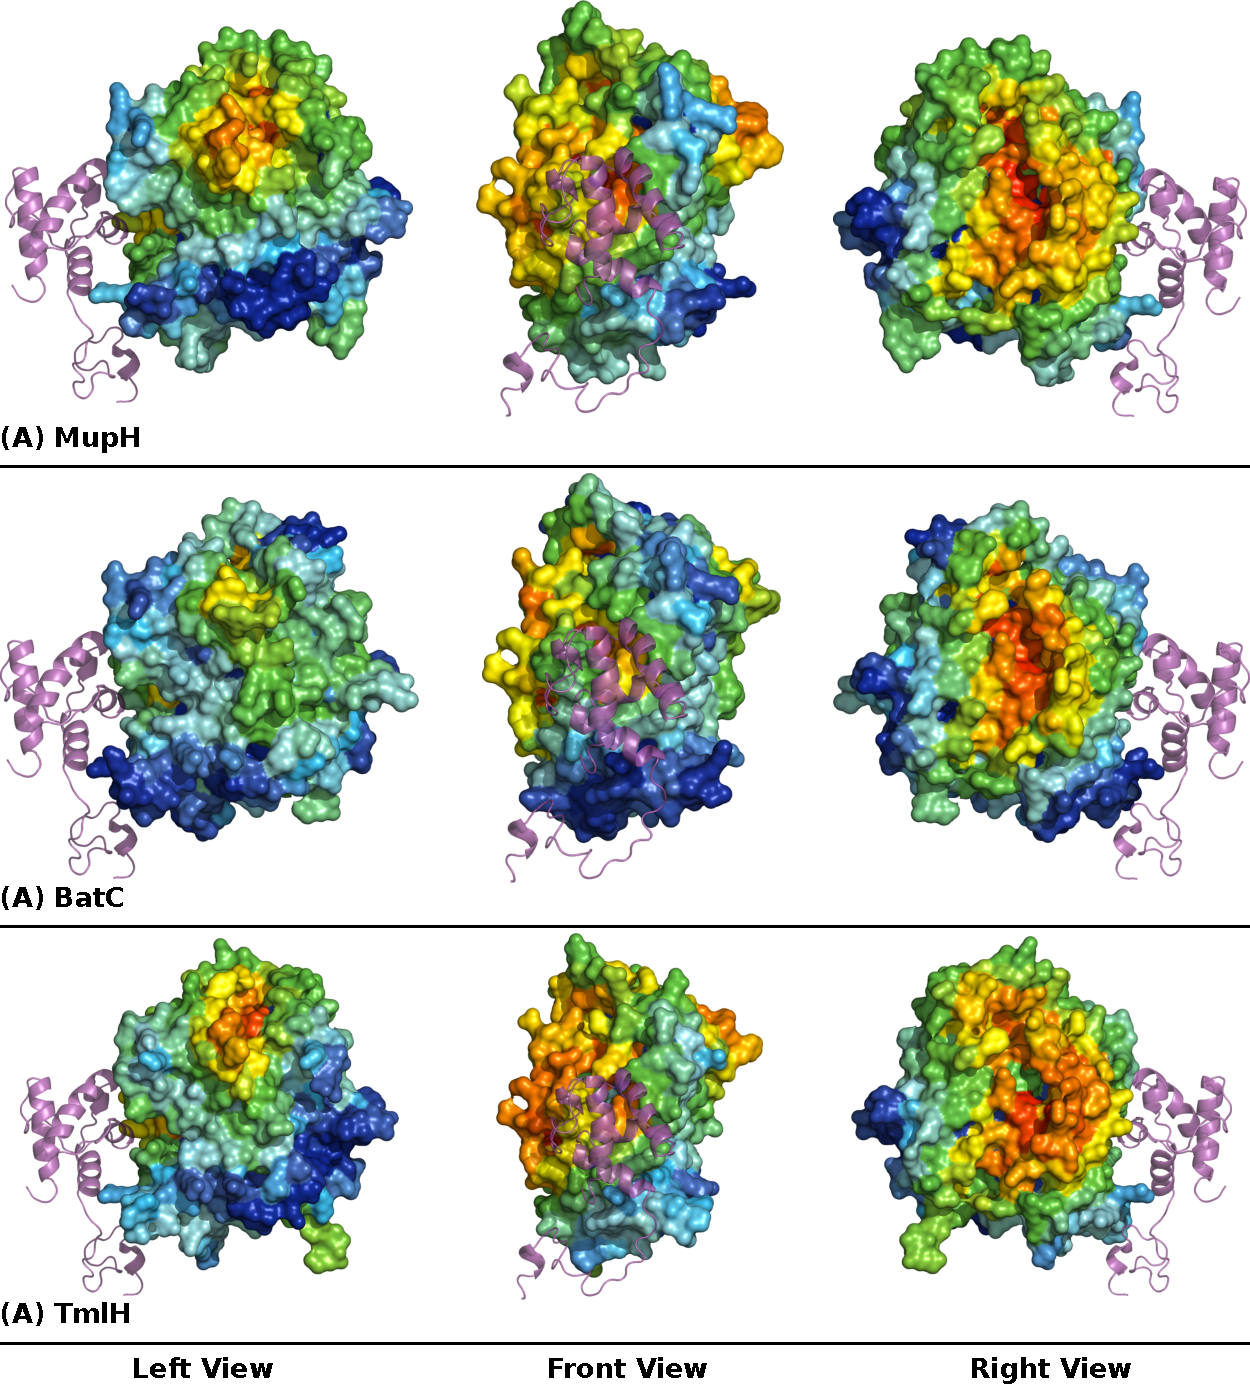
\includegraphics[width=0.9\textwidth, resolution=600, keepaspectratio=true]{graphics/PIER.pdf}}
			%\includegraphics[width=\textwidth, resolution=200, keepaspectratio=true]{graphics/polyketides.png}
			\caption[PIER analysis of MupH, BatC and TmlH.]{PIER analysis of MupH, BatC and TmlH. The different view shows the functional patch on the predicted interface of (A) MupH, (B) BatC and (C) TmlH. The left view is a 90 degree rotation anticlockwise with respect to the centre, the right view a 90 degree rotation clockwise. Residues on the surface of the MupH are coloured through the spectrum from red to blue, with red indicating predicted importance, blue lack of importance, the ACP is shown as a pink ribbon.}
			\label{fig:PIER}
			\end{figure}

		\subsubsection{Loss of function with Y to F/A mutation in ACP-mupA3a}
		\label{sec:lossoffunc}
		The above mentioned docking results which were also supported by PIER and real value evolutionary trace analysis emphasized on the importance of helix III for the formation of the ACP:MupH interaction. This helix III carried Y62 which was conserved in 95\% of the \bet-branching ACPs and it can be seen pointing towards MupH at the interacting interface and possibly making a favourable methionine to aromatic contact, methionine aromatic interaction were recently reported as important interaction in protein structure \parencite{Valley2012}. M257 was conserved in all the MupH homologue studied except TaF (myxovirescin system). Mutagenesis experiments were carried out by colleagues in Prof. Thomas group to mutate Y62 to F and A in $ \Delta $ACP-mupA3b. Phenylalanine was the most commonly occurring residue at this position in non branching ACPs. Mutating Y62 to F and A lowered the mupirocin production by three to four folds and up to ten folds respectively \parencite{Haines2013}. 
	
	\subsection{BatC complementation failure}
	\label{sec:batccomplement}
	BatC is the MupH equivalent protein from the kalamanticin cluster and it was thought that it should be able to complement MupH and produce the beta-branch in mupirocin. However, the complementation experiments showed that \textit{batC} expressed \textit{in trans} in a $ \Delta $\textit{mupH} strain greatly decreases mupirocin production. Therefore, to answer the question of why BatC did not complement MupH, bioinformatics and molecular modelling analysis was carried out using the previously modelled BatC structure. Assuming that ACP-mupA3a docks to BatC in the same orientation as it docks to MupH, the BatC structure was superimposed on to the ACP-mupA3a+MupH complex and the ACP-mupA3a+BatC model produced was analysed by CONTAC module from WhatIf package. The contacting residues found were conserved and similar to the ACP-mupA3a+MupH complex (Table \ref{tab:batcCONTAC}). 
	
	\begin{table}[htbp]
	\caption{Comparison of the contacting residues in the BatC+ACP-mupA3a pair with the MupH+ACP-mupA3a}
	\begin{center}
	\begin{tabular}{lll}
		\toprule[2pt]
		\multicolumn{1}{l}{\textbf{MupH}} & \multicolumn{1}{l}{\textbf{BatC}} & \multicolumn{1}{l}{\textbf{ACP-mupA3a}} \\ \midrule[1pt]
		R34                                & R33                                & S38                                \\
		D215                               & D214                               & L32                                 \\
		L218                               & L217                               & Y62                                 \\
		L219                               & L218                               & P65                                 \\
		L222                               & L221                               & T63                                 \\
		M257                               & M256                               & Y62                                 \\
		G260                               & G259                               & Y62                                 \\
		R267                               & R266                               & T76                                 \\ \bottomrule[2pt]
	\end{tabular}
	\end{center}
	\label{tab:batcCONTAC}
	\end{table}

	Since the contacting pairs of the residues in the BatC+ACP-mupA3a complex were found to be similar to the MupH+ACP-mupA3a complex in the CONTAC analysis it was thought that it is possible that due to superimposing the BatC structure on the MupH+ACP-mupA3a complex the analysis was biased towards the similar positions. In order to address this issue modelled BatC structure was docked to the ACP-mupA3a using the similar distance restraints as it was used for the MupH+ACP-mupA3a complex. The BatC+ACP-mupA3a docked complex came out to be almost 180 degree flip of the MupH+ACP-mupA3a complex. It was not clear why it happened as the BatC interface when superimposed on MupH+ACP-mupA3a complex was visually similar. However, in the MupH docking to ACP-mupA3b one of the clusters out of the four was similar to the BatC docking therefore, the 180 degree flip orientation was plausible but it was not dominating. In BatC docking all the complexes from both the clusters had the same orientation.  To answer this question it was thought that it might be the electrostatic potentials on the interface which are different for MupH and BatC. The electrostatic potential shows the electrostatic properties on the surface of a molecule in solution. Therefore, for two molecules to interact with each other they should have complementary electrostatic potential. Similar potentials will obviously repel each other. 
	
	To test this hypothesis the APBS \parencite{Baker2001} plugin in PyMol was used in conjunction with PDB2PQR \parencite{Dolinsky2004}. The electrostatic potentials were calculated separately for MupH, BatC and ACP-mupA3a (docked as well as BatC superimposed on MupH+ACP-mupA3a complex) and the structures were superimposed to their respective complexes for comparison. The orientation of the MupH or BatC was kept the same. Three figures were rendered for each of the complex in three different orientations for the solvent accessible and the iso surfaces. The first is the \textquotedblleft front view\textquotedblright, which shows the interacting interface as flat as possible. The other two are in left and right orientation around Y axis. The degree of rotations used were slightly different for MupH and BatC in order to highlight their interesting features as far as possible. 
	
	The electrostatic potentials for both BatC and MupH were found to be very similar with only a few subtle differences. Those few differences might be significant but it was difficult to find any difference in the specificity of MupH and BatC based on the electrostatic potentials on the protein interface. 
	
			\setlength\fboxsep{5pt}
			\setlength\fboxrule{1.5pt}
			\begin{figure} [!]
			\centering
			\fbox{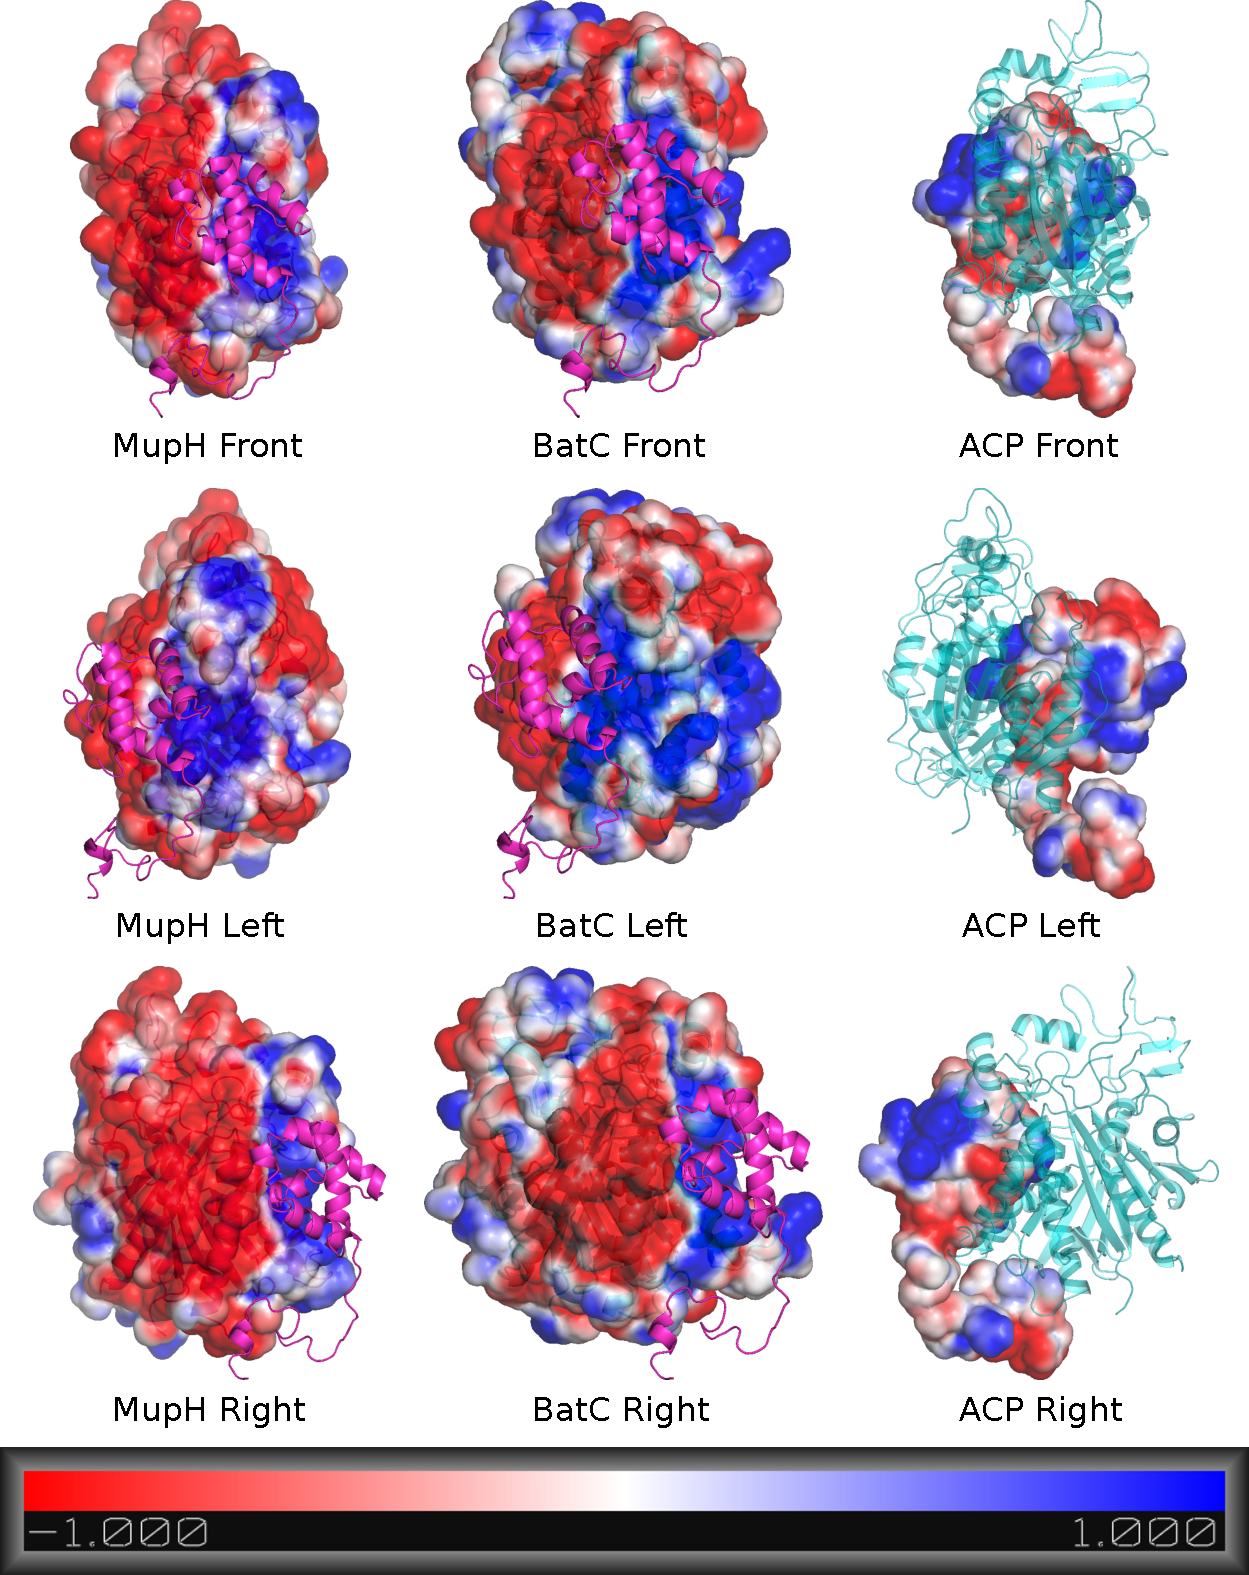
\includegraphics[width=0.9\textwidth, resolution=600, keepaspectratio=true]{graphics/solsurfmuphbatcacp.pdf}}
			%\includegraphics[width=\textwidth, resolution=200, keepaspectratio=true]{graphics/polyketides.png}
			\caption[Electrostatic potential mapped on the solution accessible surface of MupH, BatC and ACP.]{Electrostatic potential mapped on the solution accessible surface of MupH, BatC and ACP. BatC was superimposed on the MupH + ACP-mupA3a complex. The three different orientations (Front, Left and Right ) were made to clearly show the mapped potentials at the interface. The scale at the bottom shows the intensity of the negative (red) and positive (blue) potential.}
			\label{fig:solsurfmuphbatcacp}
			\end{figure}

			\setlength\fboxsep{5pt}
			\setlength\fboxrule{1.5pt}
			\begin{figure} [!]
			\centering
			\fbox{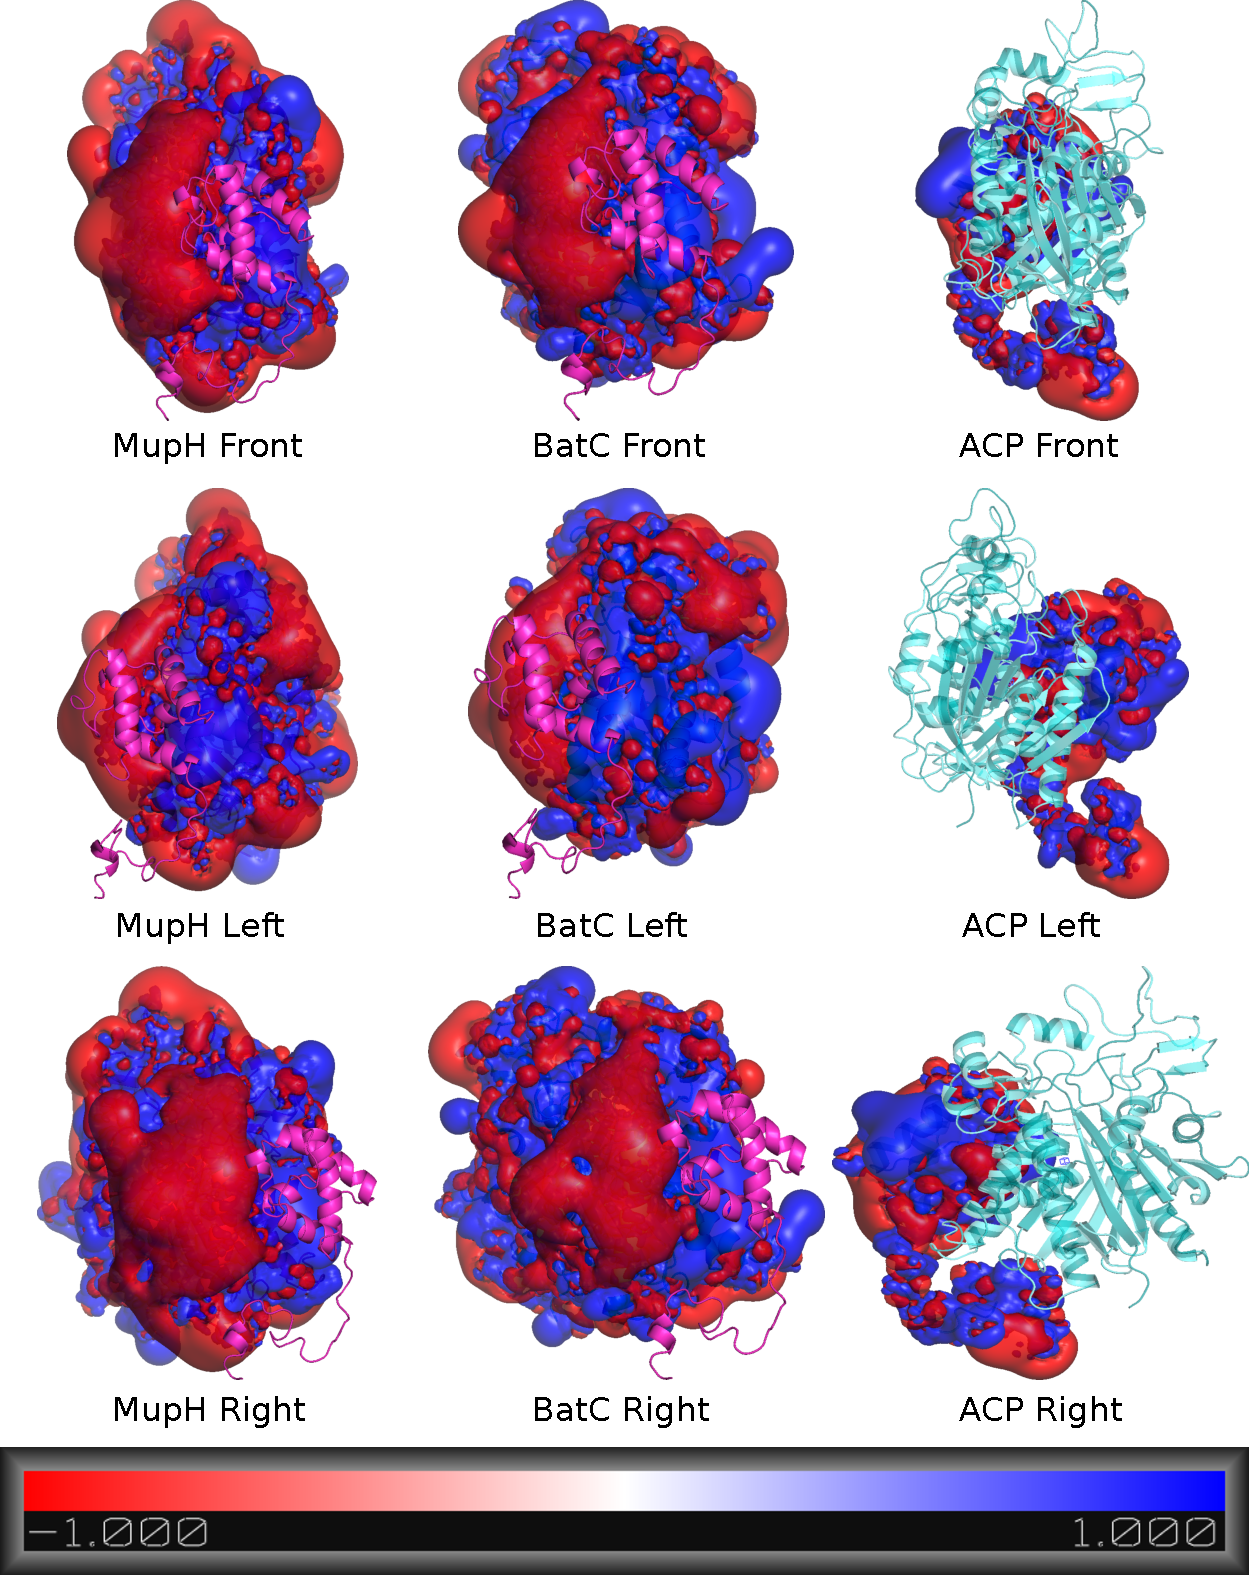
\includegraphics[width=0.9\textwidth, resolution=600, keepaspectratio=true]{graphics/isosurfmuphbatcacp.pdf}}
			%\includegraphics[width=\textwidth, resolution=200, keepaspectratio=true]{graphics/polyketides.png}
			\caption[Electrostatic potential mapped as the iso surface on MupH, BatC and ACP.]{Electrostatic potential mapped as the iso surface on MupH, BatC and ACP. BatC was superimposed on the MupH + ACP-mupA3a complex. The three different orientations (Front, Left and Right ) were made to clearly show the mapped potentials at the interface. The scale at the bottom shows the intensity of the negative (red) and positive (blue) potential.}
			\label{fig:isosurfmuphbatcacp}
			\end{figure}

			\setlength\fboxsep{5pt}
			\setlength\fboxrule{1.5pt}
			\begin{figure} [!]
			\centering
			\fbox{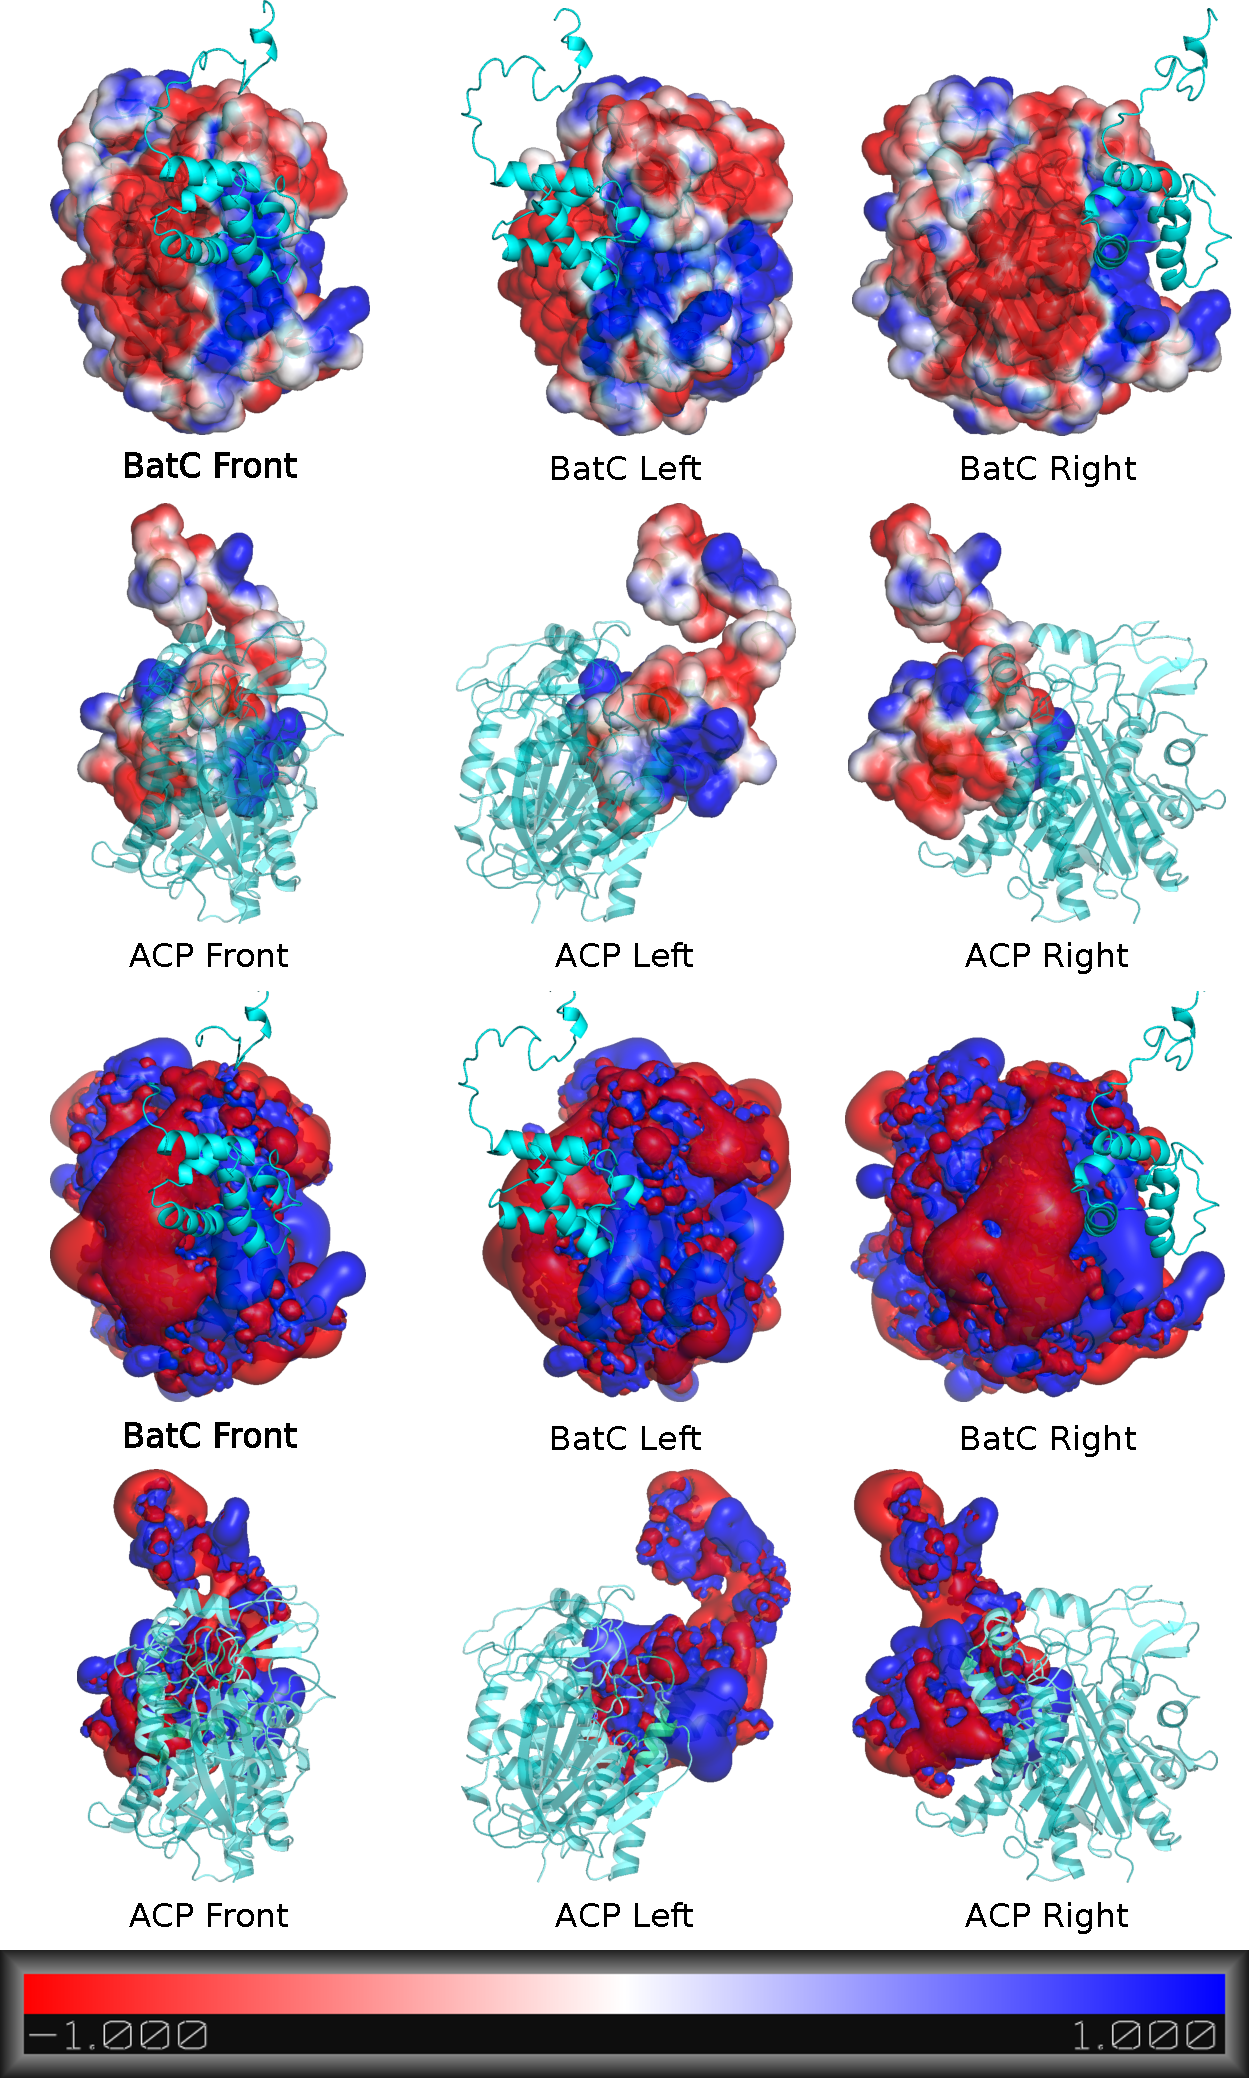
\includegraphics[width=0.8\textwidth, resolution=600, keepaspectratio=true]{graphics/dockedbatcacp.pdf}}
			%\includegraphics[width=\textwidth, resolution=200, keepaspectratio=true]{graphics/polyketides.png}
			\caption[Electrostatic potential mapped on the BatC and ACP-mupA3a docked complex.]{Electrostatic potential mapped on the BatC and ACP-mupA3a docked complex. The orientation of the BatC is kept same as that of the previous figures while the ACP can be seen as docked in almost 180 degree flip orientation. Both the solution accessible surface as well as the iso surface are shown in three different orientations (Front, Left and Right). The scale at the bottom shows the intensity of the negative (red) and positive (blue) potential.}
			\label{fig:dockedbatcacp}
			\end{figure}
		
		\subsubsection{Gain of function with L to M mutation in BatC complementation }
		\label{sec:LtoMBatC}
		The above mentioned docking and electrostatic potential analysis failed to project any striking difference between the interface of MupH with ACP-mupA3a compared to the equivalent interface between ACP-mupA3a and BatC. However, a possible answer to the riddle was in the previously determined contacting pairs of residues between the MupH/BatC and the mup ACPs. CONTAC analysis was carried out twice using a different VDW distance to define a contact each time (i.e. 0.25 \AA{} and 1.25\AA{}). Upon mapping those positions on a sequence alignment of MupH homologue from well studied systems it was revealed that the position 219 on the MupH sequence alternates between methionine and leucine an (observation made by Prof. C. M. Thomas). Interestingly TmlH, which successfully complements MupH, carried a methionine whereas BatC which failed to complement MupH carried a leucine. Looking back at the docked structure it was found that this position was at the edge of the interface and was found to be interacting with the arginine 30 of the ACP-mupA3a in 2 complexes out of 4. This methionine was not found in any of the 12 complexes with ACP-mupA3b. Figure \ref{fig:LtoMBatC} shows the position of the residues found in the CONTAC analysis as well as the key residues interacting with the ligand in the MupH active site. Mutating BatC M219L expressed in trans in the mup cluster restored mupirocin production \parencite{Haines2013}. 
		
			\setlength\fboxsep{5pt}
			\setlength\fboxrule{1.5pt}
			\begin{sidewaysfigure} [!]
			\centering
			\fbox{\includegraphics[width=0.9\textwidth, resolution=600, keepaspectratio=true]{graphics/contac.png}}
			%\includegraphics[width=\textwidth, resolution=200, keepaspectratio=true]{graphics/polyketides.png}
			\caption[Sequence alignment of MupH homologue from well studied clusters highlighting conserved interface and active site residues.]{Sequence alignment of MupH homologue from well studied clusters highlighting conserved interface and active site residues. Completely conserved interface residues with VDW distance of 0.25 \AA{} are highlighted in \colorbox{green}{light green} and residues which alternates between two residues are highlighted as \colorbox{yellow}{yellow}/\colorbox{cyan}{cyan}. Residues which are with VDW distance of 1.25 \AA{} are highlighted as \colorbox{OliveGreen}{\textcolor{white}{dark green with white text}}. The residues which are not on the interface but are in contact with the ligand are highlighted as \colorbox{magenta}{magenta}. The * symbol marks the M219.}
			\label{fig:LtoMBatC}
			\end{sidewaysfigure}		
			
\newpage	
\section{Discussion}
\label{sec:discussion}
The aim of the present work was be able to identify \bet-branching protein in PKS cluster and to elucidate the specificity mechanism involved in the ACP-HCS interaction, with a longer-term goal being to selectively introduce \bet-methylation or other HCS modifications such as cyclopropane, as part of the re-engineering of polyketide biosynthetic pathways for novel purposes.

In the mupirocin biosynthesis pathway \bet-branching is initiated by the interaction between mupA3ab tandem ACPs in module 5 of the MmpA subunit, with MupH, (the HMG-CoA homologue) in the HCS cassette. However, little was known about what governs this interaction. Sequence analysis by Dr. Anthony Haines showed that branching ACPs possess a conserved tryptophan six residues downstream of the catalytic serine but non-branching-ACPs do not. NMR studies on the tandem ACPs from the mupirocin biosynthesis pathway showed that the tryptophan and other highly conserved residues lie in the core (including L10/114, L14/118, L18/122 and F31/135) of the ACPs rather than on or near the surface. These observations raised the question as to what determines the specificity between the branching-ACPs and the MupH in the HCS cassette? Is it just the core motifs which are responsible for this specificity, if so how, or do the residues at the ACP-HCS interface also play some critical role?

In the present work, based on the previous preliminary data on the sequence analysis carried out by Dr. Anthony Hains and the NMR structures solved by Dr. Matthew Crump, further sequence analysis and molecular modelling was carried out to elucidate the specificity determinants in ACP-HCS interaction. Hidden Markov models (HMMs) were created to describe the set of branching-ACPs and the non-branching-ACPs, and were used to predict the clustering pattern between the two classes. It was seen that the HMMs were able to separate the branching-ACPs and the non-branching-ACPs into two distinct clusters with very few exceptions. The HMM models were also used to fetch more sequences from the public databases and the newly found sequences were characterised as branching or non-branching. These HMM models can be used for the annotation of newly found PKS clusters and the \bet-branching ACP HMM is now in corporated into the SMART database. The HMM models were also used to calculate the number of mutations that would be required to shift a non-branching-ACP to a branching-ACP cluster i.e. across the HMM score of 82. TmlD3-ACP from the thiomarinol cluster would require 6 mutations, with the mutation of valine to the tryptophan found conserved in the branching-ACPs being the first change.

The observation that the conserved tryptophan lies in the conserved core suggests that it might be responsible for the packing and stability of the ACP structure. Molecular dynamics simulations for the wild type and the mutant ACP in which the tryptophan was mutated to leucine showed relatively high flexibility in and around helix III in the mutant as compared to the wild type ACPs. Mutation studies carried out on T4 lysozyme structures have shown various general properties of protein folding and stability. Mutation of residues packed in the core of T4 lysozyme lowered the melting temperature of the protein whereas changes in the surface residues had little effect. These core residue changes were from \textquotedblleft hydrophobic to charged\textquotedblright \ residue, M102K (PBB ID 1L54), \textquotedblleft small to large\textquotedblright \ residue, A98F and A98W, \textquotedblleft large to small\textquotedblright \ residue, L99G (PDB ID 1QUD) and R95A disrupting various interactions made by arginine \parencite{Rennell1991, Tokuriki2009}. A \textquotedblleft large to small\textquotedblright \ residue change in the core of the T4 lysozyme seems to be similar to the W44L change in the \bet-branching ACPs. And so this suggests that we would expect W44L to destabilise the structure. Computational studies on T4 lysozyme structures also showed that the mutations primarily caused backbone shifts rather than changes in the side chain rotamers \parencite{Hurley1992, Dahiyat1997, Mooers2003}. Molecular dynamics simulations carried on \bet-branching ACPs have also showed increased flexibility in the backbone atoms of the helix III. %In T4 lysozyme structures mutations from \textquotedblleft large to small\textquotedblright \ of the rigidly buried cavity residues do not result in the collapse of protein in order to fill the space. However, mutations in more flexible cavity residues have shown the opposite \parencite{Xu1998}. In \bet-branching ACPs W44L mutant structures also does not seem to greatly affect the positions of the neighbouring packing residues. 

Docking analysis of ACPs with MupH revealed this helix III to be at the ACP-MupH interface. Helix III contains a tyrosine at the position 62 in ACP-mupA3a, which is highly conserved amongst \bet-branching ACPs, and which was found to interact with a methionine in a cleft at the MupH interface. This interaction is supported by a recent study done on methionine and aromatic residue interactions and their effect on protein structure stability \parencite{Valley2012}. Helix III in the HCS interacting ACPs was also identified to be important for halogenase activity in the curacin system \parencite{Busche2012}, also mediating an interaction with an HMG-CoA homologue. Experiments done by colleagues in Prof. Christopher M. Thomas' group mutated Y62 on helix III in ACP-mupA3a to F and A in the $\Delta$ACP-mupA3b strain and showed reduced mupirocin production  by three to four fold and ten fold respectively.  

Cross complementation experiments from Prof. Christopher M. Thomas\textquoteright group found that MupH orthologues TmlH and BatC from thiomarinol and Kalimanticin clusters respectively do restore MupH activity in an NCIMB 10586 $ \Delta $\textit{mupH} strain. However, the pseudomonic acid yield by BatC complementation is much lower than TmlH. Analysis of the predicted MupH:ACP interface residues, along with sequence analysis by Prof. Chris Thomas, suggest M219 as a specificity determining residue, being M in MupH and TmlH but L in BatC. \textit{batC} L218M was found to complement $ \Delta $\textit{mupH}, with 3 fold more antibiotic production than with wild type \textit{batC} complementation. This observation leads to a further question, if there exists a pair wise specificity between the branching ACPs and the HCS as well as a general determinant of \bet-branching ACPs the global properties of branching ACPs then replacement of ACP-mupA3ab with the ACP(s) from the kalimantacin system should either fail completely or perform poorly. However, as the mutation in the BatC helped to enhance the favourable interaction with the mupirocin ACPs analogous mutations on the kalimantacin ACP or on the mupirocin ACP should be able to help from favourable interactions between them and MupH or BatC respectively. 

Thus it can be concluded that the conserved core residues in the branching-ACPs helps in the correct packing of the branching ACPs. This packing helps the active site serine to present the substrate to the MupH active site and directing the angle of helix III which acts as another anchor at the interface. This two pin model in which the orientation of the active site serine acts as one pin and the tyrosine on the helix III another pin provides the general specificity to the ACP-MupH interaction. However, other residues found at the interface may be responsible for ACP-HCS pair wise specificity as seen in the two different ACP-HCS pairs in the myxovericin system. 











	

	
	

